\documentclass[12pt,a4paper]{book}
\usepackage[utf8]{inputenc}
\usepackage[T1]{fontenc}
\usepackage{amsmath}
\usepackage{amsfonts}
\usepackage{amssymb}
\usepackage{bbm}
\usepackage{graphicx}
\usepackage{geometry}
\usepackage{enumitem}
\usepackage{hyperref}
\usepackage{cancel}
\usepackage{forest}

\usepackage[use-files]{xsim}
\xsimsetup{path={exercises},}

\geometry{a4paper, margin=2cm}
%\usepackage{cprotect}

\usepackage{xcolor}
\definecolor{maroon}{cmyk}{0, 0.87, 0.68, 0.32}
\definecolor{halfgray}{gray}{0.55}
\definecolor{ipython-frame}{RGB}{207, 207, 207}
\definecolor{ipython-bg}{RGB}{247, 247, 247}
\definecolor{ipython-red}{RGB}{186, 33, 33}
\definecolor{ipython-green}{RGB}{0, 200, 0}
\definecolor{ipython-cyan}{RGB}{64, 128, 128}
\definecolor{ipython-purple}{RGB}{170, 34, 255}

\usepackage{listings}
\lstdefinelanguage{iPython}{
	morekeywords={access,and,del,except,exec,in,is,lambda,not,or,raise},
	morekeywords=[2]{for,print,abs,all,any,basestring,bin,bool,bytearray,callable,chr,classmethod,cmp,compile,complex,delattr,dict,dir,divmod,enumerate,eval,execfile,file,filter,float,format,frozenset,getattr,globals,hasattr,hash,help,hex,id,input,int,isinstance,issubclass,iter,len,list,locals,long,map,max,memoryview,min,next,object,oct,open,ord,pow,property,range,reduce,reload,repr,reversed,round,set,setattr,slice,sorted,staticmethod,str,sum,super,tuple,type,unichr,unicode,vars,xrange,zip,apply,buffer,coerce,intern,elif,else,if,continue,break,while,class,def,return,try,except,import,finally,try,except,from,global,pass, True, False},
	sensitive=true,
	morecomment=[l]\#,%
	morestring=[b]',%
	morestring=[b]",%
	moredelim=**[is][\color{black}]{@@}{@@},
	identifierstyle=\color{black}\footnotesize\ttfamily,
	commentstyle=\color{ipython-cyan}\footnotesize\itshape\ttfamily,
	stringstyle=\color{ipython-red}\footnotesize\ttfamily,
	keepspaces=true,
	showspaces=false,
	showstringspaces=false,
	rulecolor=\color{ipython-frame},
	frame=single,
	frameround={t}{t}{t}{t},
	backgroundcolor=\color{ipython-bg},
	basicstyle=\footnotesize\ttfamily,
	keywordstyle=[2]\color{ipython-green}\bfseries\footnotesize\ttfamily, 
	keywordstyle=\color{ipython-purple}\bfseries\footnotesize\ttfamily
}

\lstdefinelanguage{iOutput} {
	sensitive=true,
	identifierstyle=\color{black}\small\ttfamily,
	stringstyle=\color{ipython-red}\small\ttfamily,
	keepspaces=true,
	showspaces=false,
	showstringspaces=false,
	rulecolor=\color{ipython-frame},
	basicstyle=\small\ttfamily,
}

\lstnewenvironment{ipython}[1][]{\lstset{language=iPython,mathescape=true,escapeinside={*@}{@*}}%
}{%
}

\lstnewenvironment{ioutput}[1][]{\lstset{language=iOutput,mathescape=true,escapeinside={*@}{@*}}%
}{%
}

\newcommand{\mymatrix}[1]{\ensuremath{\left\downarrow\vphantom{#1}\right.\overset{\xrightarrow[\hphantom{#1}]{\text{simulations (axis 1)}}}{#1}}}
\usepackage{pifont}
\newcommand{\myendproof}{\ensuremath{\hfill\square}}
\newcommand{\HRule}[1]{\color{blue}{\rule{\linewidth}{#1}}}

%\title{Additional Material for AFM-24}
%\author{Matteo Sani}

\begin{document}

\title{\normalsize \textsc{}
		\\ [2.0cm]
		\HRule{2.0pt} \\
		\HRule{2.0pt} \\ [0.6cm]
		\LARGE \textbf{\textcolor{black}{\uppercase{lecture notes}}
		\HRule{2.0pt} \\ [0.6cm] \textcolor{black}{\Large{Additional Material for AFM Course}} \vspace*{10\baselineskip}}
		}
\date{}
\author{\textbf{Author} \\ 
		Matteo Sani \\
		A.A. 2023-2024}

\maketitle

%\begin{forest}
%[$t_0$
%	[$p_{\text{def}}$]
%	[$(1-p_{\text{def}})$
%		[$(1-p_{\text{def}})p_{\text{def}}$]
%		[$(1-p_{\text{def}})^2$
%			[$(1-p_{\text{def}})^2 p_{\text{def}}$]
%			[$(1-p_{\text{def}})^3$
%				[$(1-p_{\text{def}})^3 p_{\text{def}}$]
%				[$(1-p_{\text{def}})^4$
%					[\vdots]
%				]
%			]
%		]
%	]
%]
%\end{forest}
\chapter{Arbitrage Free Pricing Theory}
\section{Random Variables}
A variable whose value is a number determined by the outcome of a random experiment is called a \textbf{random variable}.

Random variables are very different from usual \emph{algebraic variables}:
\begin{equation*}
x^2 - 3 = 0 \implies x = \pm \sqrt{3}
\end{equation*}	
$x$ stays the same no matter how many times I solve this equation.
A random variable instead is kind of a mapping between 
\begin{equation*}
X(\omega):\Omega\rightarrow \mathbb{R}\quad \forall\omega\in\Omega
\end{equation*}
such that $X(\omega)$ represents the occurrence probability of the "outcome" $\omega$. $\Omega$ is called \textbf{sample space} and is the set of all possible future states (or outcomes) of the random process.
	
Hence the random variable $X$ will take values distributed according to the probability distribution of the random process, e.g. if $X$ represents the outcomes of rolling a \emph{fair} die $\Omega = [1,2,3,4,5,6]$ and each value has equal probability of 1/6.

\textbf{A random variable is always associated to a probability distribution.}

\subsection{Properties and Characteristics of Random Variables}		

If a random variable takes only a countable number (finite) of values, it is called \textbf{discrete}. As an example imagine when 3 coins are tossed, the number of heads obtained is a random variable, which can assume the values $\Omega=\{0,1,2,3\}$ ($\Omega$ ia a countable set).

Contrary, a random variable $X$ which can take any value between a certain interval is called \textbf{continuous}. Imagine, for example, the height of students in a particular class. It lies between 160 and 190~cm $(X = \{x|160 \leq x \leq 190\})$ and can take an infinite number of values.

Table~\ref{tab:random_variable_prop} lists the main characteristics of discrete and continuous random variables (referred to a random variable $X$ defined on a domain $\Omega$ of possible outcomes). 
\renewcommand{\arraystretch}{1.6}
\begin{table}[hbtp]
	\begin{center}
	\begin{tabular}{|c|c|} \hline
			\textbf{Discrete} & \textbf{Continuous} \\ \hline
			Probability Mass & Probability Density \\ \hline		
			$P(X=x_i)\;\forall x_i\in\Omega$ & $P(X=x)=\int_x^{x+dx}f(x)dx$ \\ \hline
			$P(x_i) \geq 0;\;\forall i$ & $f(x) \geq 0;\;-\infty < x < \infty$\\ \hline
			$\sum_{i=0}^{n} P_i = 1$ & $\int_{-\infty}^{\infty} f(x) dx = 1$\\ \hline
			\multicolumn{2}{|c|}{Cumulative Distribution} \\ \hline
			$F(x_i) = P(X<x_i) = \sum_{x<x_i} P(x)$ & $F(x) = P(X<a) = \int_{-\infty}^{a} f(x) dx$ \\ \hline
		\end{tabular}
	\end{center}
\caption{List of the main characteristics of discrete and continuous random variables.}
\label{tab:random_variable_prop}
\end{table}

If we know the distribution of a random variable, we pretty much know all is needed about it. 	
Nevertheless, when dealing with with \textit{real data}, it is quite hard to precisely know its underlying distribution, see Fig.\ref{fig:real_data}. Fortunately we can characterize it by just using a couple of important numbers called \emph{statistics}:
\begin{equation}
\begin{gathered}
\text{mean: } \mu = \mathbb{E}[X] = \int_{-\infty}^{\infty} xf(x)dx \\
\text{variance: }  
\sigma^2 = \mathbb{E}[(X-\mu)^2] =\int_{-\infty}^{\infty} (x-\mu)^2f(x)dx
\end{gathered}
\end{equation}

\begin{figure}[htbp]
\begin{center}
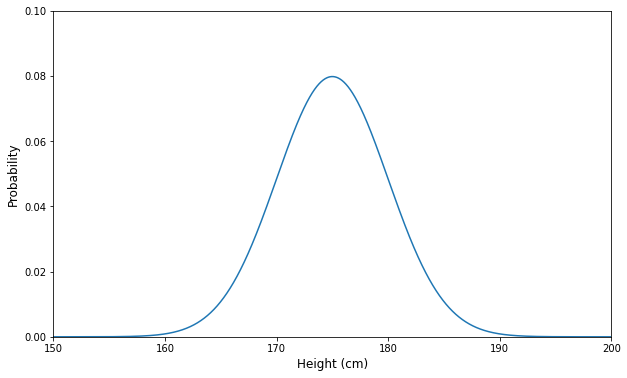
\includegraphics[height=5cm]{continouos_random_variable}
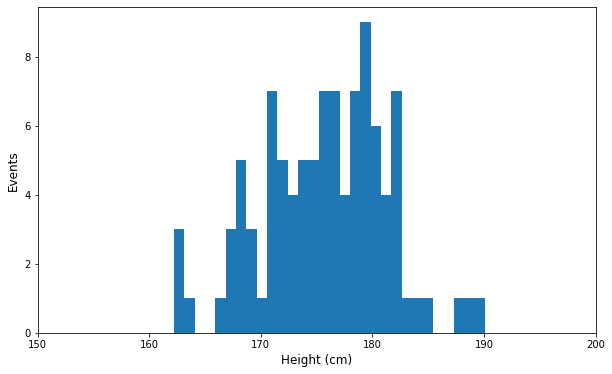
\includegraphics[height=5cm]{real_data}
\caption{Examples of a continuous random variable PDF (left) and a corresponding real life realization of the same random variable (right).}
\label{fig:real_data}
\end{center}
\end{figure} 

\subsection{Expectation and Its Properties}
Table~\ref{tab:expectation_prop} reports a list of the main properties of the expectation operator.
Essentially all of them come from the integration properties, e.g.
\begin{equation*}
	\mathbb{E}[aX] = \int_{-\infty}^{\infty} ax f(x) dx = a  \int_{-\infty}^{\infty} x f(x) dx = a\mathbb{E}[X]
\end{equation*}

\renewcommand{\arraystretch}{1.4}
\begin{table}[hbt]
	\begin{center}
		\begin{tabular}{|c|c|} \hline
			Scalar multiplication & $\mathbb{E}[aX] = a\mathbb{E}[X]$ \\ \hline
			Sums & $\mathbb{E}[X_1+\ldots +X_K] =  \mathbb{E}[X_1] +\ldots + \mathbb{E}[X_n]$ \\ \hline
			Linear combinations & $\mathbb{E}[a_1X_1+\ldots +a_KX_K] =  a_1\mathbb{E}[X_1] +\ldots + a_K\mathbb{E}[X_K]$ \\ \hline
			Expected value of a constant & $\mathbb{E}[a] = a$ \\ \hline
			Products (independent variables) & $\mathbb{E}[XY] = \mathbb{E}[X] \mathbb{E}[Y]$ \\ \hline
		\end{tabular}
	\end{center}
\caption{List of the main properties of the expectation operator.}
\label{tab:expectation_prop}
\end{table}

\section{Stochastic Processes}
Real world data is noisy (i.e. distorted), and exhibits behaviours that cannot be described by a deterministic model since it always produce the same result from  the same inputs, e.g $f(x)=x^3+2$, while the noise that "affects" real data has a random nature (Fig.\ref{fig:noisy_process}).
\begin{figure}[htbp]
	\begin{center}  
	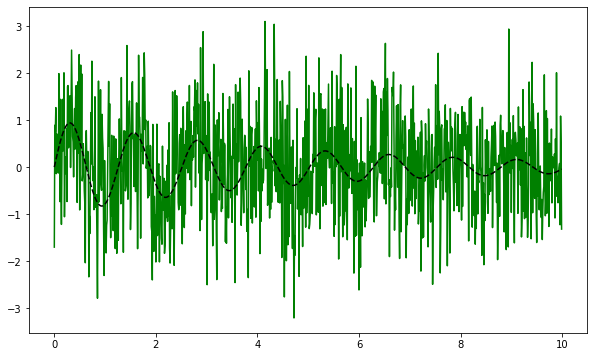
\includegraphics[height=5cm]{stochastic_process}
	\end{center}
\caption{Example of "noisy" process.}
\label{fig:noisy_process}
\end{figure}

In order to model the behavior of this kind of data (and its intrinsic uncertainty) it is needed to switch to \textbf{stochastic processes}.  
A stochastic process is a collection of random variables that is indexed by some mathematical set (usually time).

Stochastic processes are described by \emph{stochastic differential equations} (SDE):
	
\begin{equation}
\begin{aligned}
	dX(t) = \mu(t,X(t)) dt &+ \sigma(t,X(t)) dW(t) =\\  & =\underbrace{\mu(t,X(t))dt}_{\textrm{deterministic}} + \underbrace{\sigma(t,X(t)) \mathcal{N}(0,1)\sqrt{dt}}_{\textrm{stochastic}}
\end{aligned}
\label{eq:generic_sde}
\end{equation}
where $W(t)$ is called a \emph{Wiener Process} (or Brownian motion), which represents the evolution of a normally distributed random variable and whose increments are independent of everything has happened up to time $t$, for $s< t$ the stochastic variable $W(t)-W(s)$ has a Gaussian distribution $\mathcal{N}(0, t)$, i.e. the standard deviation grows with the square root of time.
Figure\ref{fig:stochastic_process_rappr} shows a schematic representation of a stochastic process.
\begin{figure}[htpb]
\begin{center}
	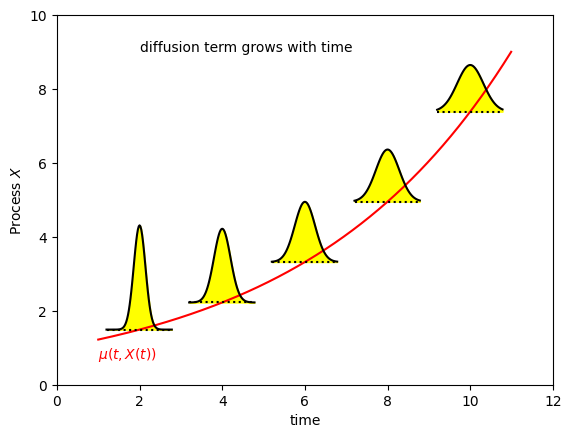
\includegraphics[height=6cm]{brownian_process}
\end{center}
\caption{Example of evolution of a stochastic process, on top of the deterministic evolution, a Gaussian distributed "noise" (Wiener process) is added.}
\label{fig:stochastic_process_rappr}
\end{figure}

Using the properties of the normal distribution we can obtain the following results for the Wiener process:
\begin{equation*}
\begin{gathered}
\mathbb{E}[\Delta W] = 0 \\
\mathbb{E}[(\Delta W)^2] = \Delta t \\
\text{Var}[\Delta W] = \Delta t \\
\text{Var}[(\Delta W)^2] = 2(\Delta t)^2 \\
\end{gathered}
\end{equation*}

The striking fact is that as $\Delta t$ tends to 0, $[(\Delta W)^2]$ goes to 0, but its variance will approach 0 much faster.
Thus, heuristically, we can say that $[(\Delta W)^2]$ looks more and more "deterministic" and in the limit we can naively say:
\begin{equation*}
\boxed{dW^2 = dt}
\end{equation*}

It is possible to interpret~\ref{eq:generic_sde} as a shorthand for 
\begin{equation*}
X(t) = X(0) + \int_0^t \mu(s,X(s)) ds + \int_0^t \sigma(s,X(s)) dW(s)
\end{equation*}
where the last term is the so-called \emph{It$\hat{o}$'s integral}.

Without entering into the details of stochastic calculus we can state the two most important properties of an It$\hat{o}$ integral:
\begin{equation*}
\begin{gathered}
\mathbb{E}\left[\int_a^b g(s) dW(s)\right] = 0 \\
\mathbb{E}\left[\left(\int_a^b g(s) dW(s)\right)^2\right] = \int_a^b\mathbb{E}[g^2(s)]ds\\
\end{gathered}
\end{equation*}

\subsection{Martingales}
With the symbol $\mathcal{F}^X_t$ it is indicated a \textbf{filtration}. It represents the information generated by the process $X$ on the interval $[0, t]$, i.e. what has happened to $X$ over that time interval. 

If the value of a stochastic variable $X$ can be completely determined given observations of its trajectories $\{X(s); 0\leq s \leq t\}$, then we can write $X\in\mathcal{F}_t^X$ and $X$ is said to be $\mathcal{F}_t^X$\emph{-measurable}.
If $Y$ is a stochastic process such that $Y(t)\in\mathcal{F}_t^X$ for all $t$ then we say that $Y$ is \emph{adapted} to the filtration $\mathcal{F}_t^X$. 

Given the information (filtration) $\mathcal{F}_t$, for any stochastic variable $X$ consider
\begin{equation*}
	\mathbb{E}[X|\mathcal{F}_t]
\end{equation*}
which represents the \textbf{conditional expectation} of $X$.
By definition it also holds that $\mathbb{E}[\mathbbm{1}_{\mathcal{F}}X] = \mathbb{E}[\mathbbm{1}_{\mathcal{F}}\mathbb{E}[X|\mathcal{F}]]$.

Given $X$ and $Y$ stochastic variables with $Y$ $\mathcal{F}_t$-measurable:
\begin{equation*}
\mathbb{E}[Y\cdot X|\mathcal{F}_t] =  Y\cdot\mathbb[X|\mathcal{F}_t]
\end{equation*}
indeed if $Y\in\mathcal{F}_t$ we know exactly its value, so in the expectation it can be treated as a constant and taken outside.
If $X$ is a stochastic variable and $s<t$ (\emph{law of iterated expectations}):
\begin{equation*}
\mathbb{E}[\mathbb{E}[X|\mathcal{F}_t]|\mathcal{F}_s] = \mathbb{E}[X|\mathcal{F}_s]
\end{equation*}

A \textbf{$\mathcal{F}_t$-martingale} is a (integrable and adapted) stochastic process which models a fair game with the following remarkable feature
\begin{equation}
\mathbb{E}[X_t|\mathcal{F}_s] = X_s
\end{equation}
so the best prediction for the future value $X_t$, given the knowledge $\mathcal{F}_s$ at time $s$ is the value at time $s$ itself, $X_s$.
		
\begin{itemize}
\item If $X_t$ is a stochastic process with diffusion coefficient $\sigma_t$, such that %which satisfies $\mathbb{E}\left[\left(\int_0^T\sigma^2_s ds\right)^{\frac{1}{2}}\right]<\infty$, and SDE 
$dX_t=\mu_t dt+\sigma_t dW_t$, then 
\begin{equation*}
X\text{ is a martingale } \iff X\text{ is drift-less } (\mu_t=0)
\end{equation*}
\item A martingale corresponds to the common notion that "a price, changes randomly" so we cannot know if it will go up or down. That is why this mathematical concept is brought into finance.
\end{itemize}	
	
\subsection{Geometric Brownian Motion (GBM)}
Trade random fluctuations deviate a stock price $S_t$ from a steady state.
The price relative change in $dt$ can be decomposed into two parts
\begin{itemize}
\item \textbf{deterministic}: the expected return from holding the stock during $dt$. It can be expressed as $\mu S_tdt$ (with $\mu$ being the expected rate of return);
\item \textbf{stochastic}: models the random changes of the market. A reasonable assumption is to equal this term to $\sigma S_t dW_t$. 
\end{itemize}

Putting all together, the resulting SDE is
\begin{equation}
\begin{gathered}
dS_t = \mu S_t dt + \sigma S_t dW_t \\
\frac{dS_t}{S_t} = d\log(S_t) = \mu dt + \sigma dW_t
\end{gathered}
\label{eq:log_normal_sde}
\end{equation}

\subsubsection{Interlude: It$\hat{o}$'s Formula}
For any given continuous and differentiable function $G(S,t)$ where S satisfies $dS=adt + bdW_t$, holds
\begin{equation}
dG = \left(a\frac{\partial G}{\partial S} + \frac{\partial G}{\partial t} + \underbrace{\frac{1}{2}b^2\frac{\partial^2 G}{\partial S^2}}_{\text{additional term}}\right)dt + b\frac{\partial G}{\partial S} dW
\label{eq:itos_lemma}
\end{equation}
			
This is essentially an extension of the \emph{Taylor series} for stochastic functions, in the expansion an extra term appears.	

Suppose $X_t$ is an stochastic process that satisfies the SDE
\begin{equation*}	
dX_{t}=\mu _{t}\,dt+\sigma _{t}\,dW_{t}
\end{equation*}.
If $f(t,x)$ is a twice-differentiable scalar function of $x$, its expansion in a Taylor series is
\begin{equation*}
df={\frac {\partial f}{\partial t}}\,dt+{\frac {1}{2}}{\frac {\partial ^{2}f}{\partial t^{2}}}\,dt^{2}+\cdots +{\frac {\partial f}{\partial x}}\,dx+{\frac {1}{2}}{\frac {\partial ^{2}f}{\partial x^{2}}}\,dx^{2}+\cdots
\end{equation*}

Substituting $X_t$ for $x$ and $dX_t$ with the SDE gives
\begin{equation*}
\begin{aligned}
df&={\frac {\partial f}{\partial t}}\,dt+{\frac {1}{2}}{\frac {\partial ^{2}f}{\partial t^{2}}}\,dt^{2}+\cdots +{\frac {\partial f}{\partial x}}(\mu _{t}\,dt+\sigma _{t}\,dW_{t})+\\
&+{\frac {1}{2}}{\frac {\partial ^{2}f}{\partial x^{2}}}\left(\mu _{t}^{2}\,dt^{2}+2\mu _{t}\sigma _{t}\,dt\,dW_{t}+\sigma _{t}^{2}\,dW_{t}^{2}\right)+\cdots
\end{aligned}
\end{equation*}

Stopping the expansion up to the first order (i.e. neglecting higher order terms in $dt^2$ and in $dt dW_t$), collecting $dt$ and $dW$ terms, and remembering that $dW^2=dt$, we obtain
\begin{equation*}
\begin{aligned}
df&={\frac {\partial f}{\partial t}}\,dt+\cancel{{\frac {1}{2}}{\frac {\partial ^{2}f}{\partial t^{2}}}\,dt^{2}}+\cdots +{\frac {\partial f}{\partial x}}(\mu _{t}\,dt+\sigma _{t}\,dW_{t})+\\
&+{\frac {1}{2}}{\frac {\partial ^{2}f}{\partial x^{2}}}\left(\cancel{\mu _{t}^{2}\,dt^{2}}+\cancel{2\mu _{t}\sigma _{t}\,dt\,dW_{t}}+\sigma _{t}^{2}\,dW_{t}^{2}\right)+\cdots =\\
&=\left({\frac {\partial f}{\partial t}}+\mu _{t}{\frac {\partial f}{\partial x}}+{\frac {\sigma _{t}^{2}}{2}}{\frac {\partial ^{2}f}{\partial x^{2}}}\right)dt+\sigma _{t}{\frac {\partial f}{\partial x}}\,dW_{t}
\end{aligned}
\end{equation*}
as required.

Back to the Geometric Brownian motion, it can be shown (see Ex.\ref{ex:gbm}) that a solution to Eq.~\ref{eq:log_normal_sde} is given by 
\begin{equation}
S_t = S_{t-1}\exp\left[\left(\mu-\frac{1}{2}\sigma^2\right)dt + \sigma\mathcal{N}(0,1)\sqrt{dt}\right] 
\label{eq:lognormal_solution}
\end{equation}

The variation in $\log(S_t)$ equals a constant (the \emph{drift} $\mu-\frac{1}{2}\sigma^2$) plus a Gaussian distributed random variable. Therefore at some time $t$
\begin{equation*}
\log S_t = \mathcal{N}\left[\left(\mu -\frac{\sigma^2}{2}\right)t, \sigma^2 t\right]
\end{equation*}
A random variable whose logarithm is normally distributed is said to be \textbf{log-normal}.
			
One of the most important properties of a log-normal distribution is to be positive definite (a mandatory characteristic for stock prices).

\section{No Arbitrage Pricing Theory}

A \textbf{portfolio} is a vector $\mathbf{\theta}\in \mathbb{R}^K$ whose $j^{th}$ component represents the number of shares of asset $A_j$ (asset $A_0$ is risk-free). It's value is
\begin{equation}
V_t(\mathbf{\theta}, \omega)=\sum_{j=1}^K\theta_jS^j_t(\omega)
\end{equation} 
where $S_t^j$ is the value of $j^{th}$ asset, and $\omega$ a market situation. A portfolio is said to be \textbf{self-financing} if its value changes only due to variations of the asset prices.

An \textbf{arbitrage} is a self-financing portfolio $\mathbf{\theta}$ such that
\begin{equation}
\begin{cases}
V_0 = 0 \\
P(V_{t}\geq 0)=1\text{ and }P(V_{t}\neq 0)>0,\,0<t\leq T
\end{cases}
\end{equation}
where $V_t$ denotes the portfolio value at time $t$ and $T$ is the time the portfolio ceases to be available on the market. 
\textbf{This means that the value of the portfolio is never negative, and guaranteed to be positive at least once over its lifetime.}

Informally, \emph{arbitrage is a way to make a guaranteed profit from nothing}, by short-selling certain assets at time $t = 0$, using the proceeds to buy other assets, and then settling accounts at time $t$. 
Arbitrage may take place when: the same asset does not trade at the same price on all markets, or two assets with identical cash flows do not trade at the same price
We are going to assume the market doesn't allow for risk-free profits with no initial investment.
Indeed arbitrage opportunities rarely exist in practice. If and when they do, gains are extremely small (not for small investors), and are typically short-lived and difficult to spot. 
\textbf{Arbitrage exclusion in the mathematical model is close enough to reality}.

\subsection{One Period Model}
Consider a bank-account $B(t)=e^{rt}$ ($r$ denote the risk-free rate) and assume today's stock price to be $S_0$. In one period of time from now, the price could be 
\begin{equation*}
\begin{cases}
S_0\cdot u = S_u \quad\text{with a certain probability $p_u$} \\
S_0\cdot d = S_d \quad\text{with a certain probability $p_d$}\\ 
\end{cases}, \text{with }(u > d)
\end{equation*}

If we want our model to \emph{forbid arbitrage opportunities}, we must impose conditions on $u$ and $d$. 
		
In case $e^r > u$, I could short the stock in $t_0$ and invest the proceeds $S_0$ into the bank account: in both future states in $t_1$, I could buy the stock back for less than my proceeds 
\begin{equation*}
S_0e^r > S_u > S_d
\end{equation*} Similarly for $e^r < d$\ldots

\begin{equation*}
\boxed{d\le e^r \le u \implies \text{no arbitrage}}
\end{equation*}

Prices of assets depend crucially on their risk as investors typically demand more profit for bearing more risk.

Therefore, today's price of a claim on a risky amount realized tomorrow will generally differ from its expected value.
Most commonly, investors are risk-averse and today's price is below the expectation, remunerating those who bear the risk.

Consequently to price assets, the calculated expected values need to be adjusted for an investor's risk preferences
Unfortunately, these adjustments would vary between investors and an individual's risk preference is very difficult to quantify.
\textbf{It turns out that, under few assumptions, there is an alternative way to do this calculation.}

\begin{equation*}
\begin{aligned}
S_0 &= \frac{S_0(u-d)e^r}{(u-d)e^r} = \frac{S_0(u-d)e^r + (S_0ud - S_0ud)}{(u-d)e^r}=\\
&= \frac{1}{e^r}\left(\frac{S_0ue^r - S_0ud}{u-d} + \frac{-S_0de^r + S_0ud}{u-d}\right)=\\
&= \frac{1}{e^r}\left(S_0u\frac{e^r - d}{u-d} + S_0d\frac{u - e^r}{u-d}\right)
\end{aligned}
\end{equation*}
The no arbitrage condition implies the following bounds
\begin{equation*}
\boxed{0\le\frac{e^r -d}{u-d}\le 1,\quad 0\le\frac{u - e^r}{u-d}\le 1}
\end{equation*}
also
\begin{equation}
\boxed{\frac{e^r -d}{u-d} + \frac{u - e^r}{u-d} = 1}
\label{eq:risk_neutral_probabilities}
\end{equation}
So we can interpret $p_u=\cfrac{e^r -d}{u-d}$ and $p_d=\cfrac{u - e^r}{u-d}$ as a \textbf{(risk-neutral) measure} ($\mathbb{Q}$).\vspace{0.3cm}
		
\subsubsection{Risk Neutral Measure}
A \textbf{probability measure} is a real-valued function that assigns probabilities to a set of events in a sample space that satisfies measure properties such as countable additivity, and assigning value 1 to the entire space.

Rewriting previous expression of $S_0$ in terms of the newly defined probabilities
\begin{equation}
S_0 = \frac{S_up_u + S_dp_d}{e^r} = e^{-r}\mathbb{E}^\mathbb{Q}[S_1]
\label{eq:risk_neutral_price}
\end{equation}
		
So the stock price is the discounted stock expectation \emph{under the chosen probability measure} at $t_1$.
	
It can be proven that there exists a \emph{risk-neutral measure} if and only \emph{if arbitrages do not exist}. 
\begin{itemize}
\item \textbf{no-arbitrage$\Rightarrow$risk-neutral measure}: requiring the model to be arbitrage-free sets conditions on $u, d$ and $e^r$ such that $p_u$ and $p_d$ define a probability measure (risk-neutral measure).
\item \textbf{risk-neutral measure$\Rightarrow$no-arbitrage}: consider an arbitrary portfolio $\theta$ and check that given the assumptions must be arbitrage-free
\begin{equation*}
V_0 = xB_0 + yS_0 = 0
\end{equation*}
This yields $x = -yS_0$.

At $t=1$ we have 
\begin{equation*}
V_1 = xB_1 + yS_1 = -yS_0e^r + yS_0Z = yS_0(Z - e^r)\quad\text{with $Z$=\{u, d\}}
\end{equation*}
To make $\theta$ an arbitrage opportunity must be $V_1\geq 0$.
			
Imagine our portfolio has $y > 0$ then there is arbitrage if and only if $u - e^r \geq 0$ and $d - e^r \geq 0$
which can not happen according to the assumptions. 
			
Thus, if $y > 0$ \emph{the portfolio is not an arbitrage one}. The case $y < 0$ is treated in the same way.
\myendproof
\end{itemize}

But what does it mean "risk-neutral measure" ?
The \emph{risk-neutral measure} is agreed upon by the market as a whole just as a consequence of no arbitrage assumption.
In other words it is nothing more than an \emph{implied probability distribution}.
Implied from observable prices of tradable instruments, and used to determine \emph{objective fair prices} for an asset or financial instrument. Probabilities are assessed with the risk taken out of the equation, so it doesn’t play a factor in the anticipated outcome.
By contrast, if you tried to estimate the anticipated value of a stock based on how likely it is to go up or down, considering unique factors or market conditions that influence that specific asset, you would be including risk into the equation and, thus, would be looking at \emph{real or physical probability}.

\subsubsection{Market Completness}
A \emph{contingent claim} (financial derivative) is any stochastic variable $X$ of the form $X=\Phi(Z)$, where $Z$ is a stochastic process driving the stock price process above. 
The function $\Phi$ is called the \emph{contract function}.

As an example consider an European call option on the stock $S$ with strike $K$, (assume $S_0d < K < S_0u$)
\begin{equation*}
X = \begin{cases}
\Phi(u) = S_0 u - K\\
\Phi(d) = 0
\end{cases}
\end{equation*}
We aim at determine the "fair" price $\Pi(t; X)$, if it exists, for a given contingent claim $X$.

A portfolio $\mathbf{\theta}$ in the assets $A$ is a \textbf{replicating portfolio} for a contingent claim $X$ if
\begin{equation}
V_t = \sum_{j=1}^K \theta_j S_t^j(\omega_i)\quad\forall i=1,2,\ldots,N
\end{equation}
where $V_t$ is the asset price at time $t$.
If all claims (assets) can be replicated the market is said to be \textbf{complete}.
From a financial point of view, there is no difference between holding the claim and holding the portfolio, no matter what happens on the stock market, the value of the claim and of the stock will be the same.
	
Conversely, if the market is complete, and if the \emph{unique} risk-neutral measure $\mathcal{Q}$ gives positive probability to every market scenario $\omega$, then for every derivative security there is a replicating portfolio.
\begin{itemize}
\item \textbf{complete market$\Rightarrow$no-arbitrage}: consider the replicating portfolio $\theta$ of a contingent claim $X$. If $\Pi(0; X) < V_0^\theta$ then at time $t=0$ we buy the claim, sell the portfolio and put the proceeds $V_0^\theta-\Pi_0$ in the bank so the net position is 0. At $t=1$ we will receive the claim payoff $X$ and will have to pay $V_1^\theta =X$  to the holder of the portfolio. This cancels but we still have $e^r(V_0^\theta-\Pi_0)>0$ in the bank. Thus we have an arbitrage. Similarly $\Pi(0; X) > V_0^\theta$.
\item \textbf{no-arbitrage$\Rightarrow$complete market}: fix and arbitrary claim $X$ with contract function $\Phi$ and a portfolio such that
\begin{equation*}
\begin{cases}
V_1 = x e^r + yS_0u = \Phi(u)\\
V_1 = x e^r + yS_0d = \Phi(d)
\end{cases}
\end{equation*}
			
Since our model assume $d<u$ there exists a \textbf{unique} solution
\begin{equation}
\begin{aligned}
x &= e^{-r}\cfrac{u\Phi(d)-d\Phi(d)}{u-d} \\
y &= \cfrac{1}{S_0}\cfrac{\Phi(u)-\Phi(d)}{u-d}
\end{aligned}
\label{eq:replica_portfolio_value}
\end{equation}

Under the conditions which makes our model arbitrage-free, there exists a martingale (risk-neutral) measure and the free arbitrage price of a contingent claim $X$ is given by 
\begin{equation*}
\Pi(0; X) = e^{-r}\mathbb{E}^{\mathbb{Q}}[X]
\end{equation*} 
The martingale measure $\mathbb{Q}$ is uniquely identified by~\ref{eq:risk_neutral_probabilities}.
		
Indeed, the market is complete, so from the replicating portfolio we know that $\Pi(0;X) = V_0$ and using~\ref{eq:risk_neutral_probabilities} and~\ref{eq:replica_portfolio_value} we can explicitly calculate the price as
\begin{equation*}
\Pi(0;X) = e^{-r}\left[\cfrac{e^r-d}{u-d}\Phi(u)+\cfrac{u-e^r}{u-d}\Phi(d)\right] = e^{-r}\left[q_u\Phi(u)+q_d\Phi(d)\right]
\end{equation*}
the expected value, under the martingale measure.
Such a price is given by the expectation of the discounted payoff under the measure $\mathbb{Q}$.
\end{itemize}
\myendproof

\subsubsection{No Arbitrage Pricing Summary}
\begin{itemize}
\item The market is free of arbitrage if (and only if) there exists an \textbf{equivalent martingale measure} (EMM) (i.e. a risk-neutral measure).
\item The market is complete if and only if the martingale measure is unique.
\item In a complete and arbitrage-free market the price of any derivative is uniquely given, either by the value of the associated replicating strategy, or by the expectation of the discounted payoff under the risk-neutral measure
\begin{equation}
\Pi_t = \mathbb{E}^{\mathbb{Q}}[D(t,T)V_A|\mathcal{F}_t]
\label{eq:risk_neutral_pricing}
\end{equation}
\end{itemize}

\section*{Exercises}
\begin{exercise}[subtitle={Geometric Brownian Motion}]
\label{ex:gbm}
Show that 
\begin{equation*}
S_t = S_{t-1}\exp\left[\left(\mu-\frac{1}{2}\sigma^2\right)dt + \sigma\mathcal{N}(0,1)\sqrt{dt}\right] 
\end{equation*}
is a solution of the stochastic differential equation
\begin{equation*}
dS_t = \mu S_t dt + \sigma S_t dW_t \\
\end{equation*}
\end{exercise}

\begin{solution}
Let's apply the Ito's expansion to $G=\log(S_t)$ 
\begin{equation*}
\frac{\partial G}{\partial S}=\frac{1}{S_t},\;\frac{\partial G}{\partial t}=0,\;\frac{\partial^2 G}{\partial S^2}=-\frac{1}{S_t^2}
\end{equation*}

Substituting back into It$\hat{o}$'s lemma and taking $a$ and $b$ values from the SDE for $S$
\begin{equation*}
dG = \left(a\frac{\partial G}{\partial S} + \frac{\partial G}{\partial t} + \frac{1}{2}b^2\frac{\partial^2 G}{\partial S^2}\right)dt + b\frac{\partial G}{\partial S} dW
\end{equation*}

\begin{equation*}
d(\log S_t) = \left[\mu S_t\frac{1}{S_t} + \frac{1}{2}\sigma^2S_t^2\left(-\frac{1}{S_t^2}\right)\right]dt + \sigma dW
\end{equation*}

\begin{equation*}
\log(S_t) - \log(S_{t-1}) = \log\frac{S_t}{S_{t-1}}=\left(\mu - \frac{1}{2}\sigma^2\right)dt + \sigma dW 
\end{equation*}	

\begin{equation*}
S_t = S_{t-1}\exp\left[\left(\mu-\frac{1}{2}\sigma^2\right)dt + \sigma\mathcal{N}(0,1)\sqrt{dt}\right] 
\end{equation*}
\end{solution}

\begin{exercise}[subtitle=Martingale, tags={sde}]
Consider the process $Y(t) = 2^{W(t)}$, where $\{W(T):t\geq 0\}$ is a standard Brownian motion. 
Is this a martingale ?
\end{exercise}
\begin{solution}
With $g(t)=2^{W(t)}$, we find:
\begin{equation*}
dg(t) = \ln2\cdot 2^{W(t)}dW(t) +\cfrac{(\ln2)^2}{2}2^{W(t)}dt
\end{equation*}
Note that $g, g_{x}, g_{xx}$ exist and are continuos. 
Due to the appearance of a $dt$-term, the process is not a martingale.	
\end{solution}

\begin{exercise}[subtitle={Stochastic Differential Equation}, , tags={sde}]
Show that the exponential SDE
\begin{equation*}
	dX_t = A_t X_tdW_t,\quad X_0=x_0
\end{equation*}
has the following solution
\begin{equation*}
	X_t = x_0 e^{-\frac{1}{2}\int_0^t A_0^2 ds+\int_0^t A_s dB_s}
\end{equation*}
\textbf{Hint:} Apply Ito's formula to $f(Y_t)$ where $f(x)=x_0 e^x$ and $Y_t=-\frac{1}{2}\int_0^t A_s^2 ds + \int_0^t A_s dB_s$
\end{exercise}
\begin{solution}
	The SDE can be expressed as $d(\ln(X_t)) = \cfrac{dX_t}{X_t} = A_t dW_t$ where we have changed to the variable $Y_t = \ln(X_t)$. Applying Ito's formula to $Y_t$ 
	\begin{equation*}
		dY_t = \left[a\cfrac{\partial Y}{\partial X} + \cfrac{\partial Y}{\partial t} + \frac{1}{2}b\cfrac{\partial^2 Y}{\partial X^2}\right]+ b\cfrac{\partial Y}{\partial X}dW_t
	\end{equation*}
	but $a=0, \frac{\partial Y}{\partial t}=0, b=A_tX_t, \frac{\partial Y}{\partial X}=\frac{1}{X}, \frac{\partial^2 Y}{\partial X^2}=-\frac{1}{X^2}$, so
	\begin{equation*}
		dY_t = \left[\cancel{a\cfrac{\partial Y}{\partial X}} + \cancel{\cfrac{\partial Y}{\partial t}} - \frac{1}{2}A_t^2 \cancel{X_t^2}\cfrac{1}{\cancel{X^2}}\right]+ A_t\cancel{X_t}\cfrac{1}{\cancel{X_t}}dW_t = -\frac{1}{2}A_t^2 + A_t dW_t
	\end{equation*}
	Integrating and considering the initial condition given by the problem
	\begin{equation*}
		\begin{gathered}
			\ln\left(\frac{X_t}{X_0}\right) = -\frac{1}{2}\int_0^t A_s^2 ds + \int_0^tA_s dW_s \\
			X_t = X_0 \exp\left(-\frac{1}{2}\int_0^t A_s^2 ds + \int_0^tA_s dW_s \right)
		\end{gathered}
	\end{equation*}
This solution is known as the exponential martingale solution.
\end{solution}


\chapter{Monte Carlo Simulation}

\section{Stochastic Simulation}
In science, we are often more interested in the distribution of a set of outcomes rather than a single event. This may be the probability distribution of a molecule diffusing a specific distance as a function of time, or the price change of a very exotic derivative.

Stochastic simulations allow us to generate a series of experiments on a system in which one or more steps is governed by random chance. These simulations often boil down to "flipping a coin" to dictate if said step will occur or not.
To get a sense of the probability distribution of some outcome, we often have to simulate the process thousands of times. This means that we need to know how to make our computers do the heavy lifting.

\section{The Algorithm}
A Monte Carlo simulation is a mathematical technique that simulates the range of possible outcomes for an uncertain event.

These predictions are based on an estimated range of values instead of a fixed set of values and evolve randomly.

Essentially the process is simulated by replacing every source of uncertainty by random numbers sampled from appropriate distributions (PDF). 

Monte Carlo simulations use a probability distribution for any variable that has inherent uncertainty, it recalculates the results many times, using a different set of random numbers each time. This process generates many probable outcomes, which become more accurate as the number of inputs grows.
Note that depending upon the number of uncertainties and their ranges, a Monte Carlo simulation could involve thousands or even millions of recalculations before it is completed.

The Monte Carlo method has been described as "faking it a billion times until the reality emerges". It relies on the assumption that many random samples mimic patterns in the total population.

Although they might vary from case to case, the general steps to a Monte Carlo simulation are as follows:
\begin{itemize}
\item Determine the mathematical model.
\item Pick the stochastic variables, and determine an appropriate probability distribution (PDF) for each and their range of variability $\Omega$.
\item Run the random variables through the mathematical model to perform many simulations (or experiments).
\item Aggregate the results, and determine the mean, standard deviation and variant to determine if the result is as expected. Alternatively visualize the result distribution on a histogram.
\end{itemize}

\subsubsection{An Example}

Imagine to simulate the results of rolling a die: the only variable is the die outcome, so $\Omega =1,2,3,4,5,6$ and the outcome probability is a uniform distribution (i.e. we are using a fair die and outcomes are equiprobable). Hence the simulation consists of sampling uniform distributed integers between 1 and 6.

\subsection{Array in \texttt{python}}

A convenient way of storing the results of a Monte Carlo simulation in \texttt{python} is using \texttt{numpy.array} objects. 

These are a faster replacement for native \texttt{list} objects which are implemented in \texttt{C} language thus overtaking the usual performance bottlenecks of the \texttt{python} language. 

One of the most interesting feature of \texttt{numpy.array} is the so called \emph{vectorialization}, which is the capability of applying a certain operation to each element of the array without expliciting the for-loop on them.

The following example shows the result of applying the logarithm to a list of numbers first in the "traditional" way then using vectorialization.
\begin{ipython}
import numpy as np
import math 

data = [1.14, 13.45, 7.7, 10, 2.75]
for i in range(len(data)):
	print (math.log(data[i]))
	
data_vec = np.array(data)
print (np.log(data_vec))
\end{ipython}

When dealing with multidimensional arrays you need to pay attention to the \emph{axis} you want to perform such operations.

In fact imagine a $m\times N$ matrix representing $N$ simulation of the variation of a Brownian motion $dW$ for $m$ time steps.

\begin{equation}
	\text{\tiny time (axis 0)}\mymatrix{\begin{pmatrix}
			dW_0(t_0) & dW_1(t_0) & \cdots & dW_N(t_0) \\
			dW_0(t_1) & dW_1(t_1) & \cdots & dW_N(t_1) \\
			\vdots  & \vdots  & \ddots & \vdots  \\
			dW_0(t_m) & dW_1(t_m) & \cdots & dW_N(t_m)
	\end{pmatrix}}
\label{numpy_array}
\end{equation}
If I would like to get each realization of $W$ I have to sum all the changes $dW$ for each simulation (hence sum up along the "time" axis). 

This can be done by using \texttt{numpy.cumsum} (cumulative sum) function specifying that the sum has to be done along \texttt{axis=0}. In the following simple example we have 3 simulations and 2 time steps.

\begin{ipython}
import numpy as np

dW = np.array([[1,2,3],[4,5,6]])
print (f"Matrix dimensions: {dW.shape}")
print (dW)
W = np.cumsum(dW, axis=0)
print (f"sum along axis 0: \n{W}")
\end{ipython}
\begin{ioutput}
Matrix dimensions: (2, 3)
[[1 2 3]
[4 5 6]]
sum along axis 0: 
[[1 2 3]
[5 7 9]]
\end{ioutput}

Then, for example, you can mediate over the simulations to get the mean path as a function of time. In this case it can be used the \texttt{numpy.mean} function specifying that the operation has to be done along \texttt{axis=1}

\begin{ipython}
Wm = np.mean(W, axis=1)
print (f"mean path: \n{Wm}")
\end{ipython}
\begin{ioutput}
mean path: 
[2. 7.]
\end{ioutput}

The output has correctly length 2, since there is just one path, i.e. the mean path, made of two time steps.

\subsection{Simulating Stochastic Differential Equations}

Consider a generic stochastic differential equation (SDE)

\begin{equation}
dX(t) = \mu(t,X(t))dt + \sigma(t,X(t))dW(t)
\label{eq:sde}
\end{equation}

The Monte Carlo simulation of such a process can be carried out according to the \emph{Euler scheme} as follows: consider the value of $X$ at time $t=t_i$, the value $X(t_{i+1})$ is evaluated directly \emph{discretizing}  the dynamics of X (Eq.~\ref{eq:sde}). Set $\Delta t = t_{i+1} - t_{i}$, and sample from a standard normal $z = \mathcal{N}(0,1)$ in order to "evolve" the stochastic term $dW$, then 
\begin{equation}
X(t_{i+1}) = X(t_i) + \mu(t_i,X(t_i))\Delta t + \sigma(t_i,X(t_i))\sqrt{\Delta t}z
\end{equation}

In the specific case of a simple Brownian motion the dynamics is given by
\begin{equation}
dW = \sqrt{dt}\mathcal{N}(0,1)
\end{equation}
so
\begin{equation}
W(t+dt) = W(t) + \sqrt{dt}\mathcal{N}(0,1)
\end{equation}
or, for the entire realization
\begin{equation}
W(t) = \sum_{t_0}^{t} \sqrt{dt}\mathcal{N}(0,1)
\end{equation}

\section*{Exercises}
\begin{exercise}[subtitle={Central Limit Theorem  (\texttt{python})}]
Using a Monte Carlo simulation of coin flip check the Central Limit Theorem:
\begin{itemize}
\item the distribution of the mean of repeated experiments is distributed like a Gaussian around the true mean;
\item as the number of experiments (simulations) increase the precision of the estimate increase.
\end{itemize}
\end{exercise}

\begin{exercise}[subtitle={Monte Carlo}]
You have determined the value of an interest rate derivative with a Monte Carlo simulation involving 50 scenarios which results in a contract value of 1.2 M€ $\pm$ 5\%. Unfortunately your boss ask you to determine more precisely the derivative value. If you have to meet him in 1 hour and each simulation lasts about 2.5 sec., what is the highest precision you can achieve ?
\end{exercise}
\begin{solution}
Given you have to answer in 1 hour, you can run at most: $\frac{3600}{2.5}=1440$ experiments. Since the result precision scale as the square root of the number of simulations
\begin{equation*}
\textrm{new uncertainty} = 0.05 \cdot \sqrt{\frac{50}{1440}} \approx 0.01
\end{equation*}
\end{solution}

\begin{exercise}[subtitle={1D Random Walk (\texttt{python})}, label={ex:2.2}]
Code a function that simulate a 1D random walk. 

\textbf{Note: } the Random Walk in one dimension is a model for each process which have simple binary outcomes.
The 1D random walk can be used to model how a gambler plays a game such as roulette in a casino. The idea in such games is that the gambler places a small stake on each game (say 1€). When the game is played the gambler will either loose and the total amount of money he has will thus decrease by one unit, or alternatively, he will win the game and in that case he wins back his stake and a prize, which we will set as 1€. As you can see if the gambler repeats this process of staking money and playing the amount of money he has will undergo a random walk in one dimension, since the outcome will be either 1 or -1.
\end{exercise}

\begin{solution}
\begin{ipython}
import numpy as np
import matplotlib.pyplot as plt

np.random.seed(10)
def random_walk_1d(startpoint, nsteps, p):
    X = np.zeros(shape=(nsteps,))
    X[0] = startpoint
    games = np.random.random(size=nsteps-1)
    X[1:] = np.where(games>p, 1, -1)
    return np.cumsum(X)

X = random_walk_1d(0, 100, 0.5)

plt.plot(X)
plt.show()
\end{ipython}
\end{solution}

\begin{exercise}[subtitle={Simulating a Gambler (\texttt{python})}]
Write a function called gambler that simulates this procedure, taking three arguments:

Determine with a simulation the probabilities whether the gambler leaves the casino with zero or with $N$€.
Essentially we start the gambler with $X$€ and simulate the process of him playing the game only stopping once he has reached one of the two thresholds.

\begin{itemize}
\item \texttt{start}: the amount of money the gambler starts with; \item \texttt{n}: the target amount of money that the gambler wants to win;
\item \texttt{p}: the probability of winning each individual game the gambler plays.
\end{itemize}

\textbf{Note: } importantly there is a difference between the gambler and the 1D random walk, however. The gambler usually only has a finite amount of money to gamble with. If he looses a large number of games he is therefore forced to stop playing. Similarly, the gambler may also have some target for how much money he would like to win. In other words, he should have some figure $N$€, which is more than the amount of money he entered the casino with. He will stop gambling once he has $N$€ in his pocket.
\end{exercise}
\begin{solution}
\begin{ipython}
# It should be implemented an exit strategy against infinite loop
# The gambler cannot play for an infinite amount of time

def random_walk_with_stop(startpoint, p, N):
    X = [startpoint]
    while True:
        game = np.random.random()
        if game < p:
            X.append(X[-1] + 1)
        else:
            X.append(X[-1] - 1)
        if X[-1] <= 0:
            return 0
        elif X[-1] >= N:
            return 1

simulations = 10000
outcomes = []
for _ in range(simulations):
    outcomes.append(random_walk_with_stop(100, 0.5, 120))

print (f"Probability to hit upper limit: {sum(outcomes)/simulations}")
\end{ipython}
\end{solution}

\begin{exercise}[subtitle={Spin to End (\texttt{python})}]
Write another function that simulates the changes in the amount of money the gambler has and that returns the number of spins of the wheel that take place.

\textbf{Note: } we can also use simulation to determine how many spins of the wheel the gambler will play before leaving the casino (i.e. \emph{hitting time}).
In other words we want to calculate the number of steps the random walk takes before arriving in one of the two threshold states.
\end{exercise}
\begin{solution}
\begin{ipython}
def random_walk_with_stop_for_steps(startpoint, p, N):
    games = 0
    X = [startpoint]
    while True:
        game = np.random.random()
        games += 1
        if game < p:
            X.append(X[-1] + 1)
        else:
            X.append(X[-1] - 1)
        if X[-1] <= 0 or X[-1] >= N:
            return games

simulations = 10000
games = []
for _ in range(simulations):
    games.append(random_walk_with_stop_for_steps(100, 0.5, 120))

print (np.mean(games))
\end{ipython}
\end{solution}

\begin{exercise}[subtitle={Martingale Game}]
Suppose you play the following series of games. In game $i, i = 1, 2,\ldots$, you bet \$1 and roll a fair die. If the outcome is $\{1,2\}$ you win \$1, if it is $\{3,4\}$ nothing happens, and if the outcome is $\{5,6\}$ you lose \$1.

Prove that the random process representing the gamer gain is a martingale.
Also using Monte Carlo simulation implement the game described in the text and check that the expected gain is indeed null.
\end{exercise}
\begin{solution}
Let $X_i$ be a random variable representing the amount of money you win or lose in bet $i$, this kind of game is said to be \emph{fair} since

$$\mathbb{E}[X_i]= \sum_{\Omega}p(\omega)\cdot x(\omega) = \frac{2}{6}\cdot 1 + \frac{2}{6}\cdot 0 + \frac{2}{6}\cdot -1 = 0\;\forall i$$
so no unbalance between losses or wins.

Now define another random variable $Z_n = \sum_{i=1}^{n} X_i$, i.e. the amount of money held at the $n$-th game.

$Z_n$ is a martingale and $\mathbb{E}[Z_n|X_1,\ldots, X_{n-1}] = Z_{n-1}$.

\begin{equation*}
	\begin{aligned}
		\mathbb{E}[Z_n|X_1,\ldots, X_{n-1}] &= \mathbb{E}[X_1 +\ldots + X_n|X_1,\ldots, X_{n-1}] \\
		& = \underbrace{\mathbb{E}[X_1|X_1,\ldots, X_{n-1}]}_{X_1} + \ldots + \underbrace{\mathbb{E}[X_{n-1}|X_1,\ldots, X_{n-1}]}_{X_{n-1}} + \underbrace{\mathbb{E}[X_n|X_1,\ldots, X_{n-1}]}_{\mathbb{E}[X_n]=0} \\
		& = \mathbb{E}[X_1|X_1,\ldots, X_{n-1}] + \ldots + \mathbb{E}[X_{n-1}|X_1,\ldots, X_{n-1}] + 0 = Z_{n-1}
	\end{aligned}
\end{equation*}

\begin{ipython}
import matplotlib.pyplot as plt
import numpy as np

K0 = 10
simulations = 100000
games = 500

np.random.seed(1)
K = np.zeros(shape=(simulations, games))
for s in range(simulations):
    K[s, :] = np.random.randint(1, 7, size=games)
    K[s, :] = np.where(K[s, :]<3, -1, K[s, :])
    K[s, :] = np.where(K[s, :]>4, 1, K[s, :])
    K[s, :] = np.where((K[s, :]<5)&(K[s, :]>2), 0, K[s, :])
    K[s, :] = np.cumsum(K[s, :])

for s in range(10):
    p = plt.plot(K0 + K[s, :])

mean = np.mean(K[:, -1])
std = 1.96*np.std(K[:, -1])/np.sqrt(simulations)
plt.text(20, 42, f"Expected gain: {mean:.2f} +- {std:.2f}", fontsize=20)
plt.grid(True)
plt.xlim(0, games)
plt.xlabel("games", fontsize=14)
plt.show()
\end{ipython}
\end{solution}

%\begin{exercise}[subtitle=2D Random Walk  (\texttt{python})]
%An unbiased random walk (in any number of dimensions) is another example of a martingale.
%
%In higher dimensions, the set of randomly walked points has interesting geometric properties. In fact, one gets a discrete \emph{fractal}, that is, a set that exhibits stochastic self-similarity on large scales.
%
%Implement a 2D random walk simulation and plot one possible realization.
%\end{exercise}

\begin{exercise}[subtitle={Brownian Motion (\texttt{python})}]
Simulate a couple of realization of a Brownian motion process with initial value 0.
Figure~\ref{fig:brownian_motion} reports two realization of the Brownian motion simulated according to the Euler scheme.
\end{exercise}

\begin{exercise}[subtitle={Geometric Brownian Motion  (\texttt{python})}]
Using the Euler scheme simulate the 4-months (with daily steps) evolution of a Geometric Brownian Motion stochastic process with initial value $S_0=100$, $\mu=0.005$, and $\sigma=0.05$.
\end{exercise}

\begin{exercise}[subtitle={Geometric Brownian Motion  (\texttt{python})}]
This \href{https://github.com/matteosan1/advanced_financial_modeling/raw/master/input_files}{file} contains a thousand 10-day realizations (with 0.1 day step) of historical price data of a single asset, assume that all the time series are different realizations of the same stochastic process.
\begin{enumerate}
\item Make two figures: the first should contain one realization as a function of time, in the second plot the first 50 realizations together as a function of time (\emph{label the axes appropriately}).
\item In two separated plots report the mean and the variance of the stock prices as a function of time (\emph{label the axes appropriately}).
\item Perform the variable change $X_{n+1}=\log\left(\cfrac{S_{n+1}}{S_n}\right)$ on $S_{n+1} = S_ne^{(\mu-0.5\sigma^2)\Delta t + \sigma\sqrt{\Delta t}Z}$ to rewrite the model into a simpler form. 
	\begin{enumerate}
	\item Is the resulting dynamics linear ? Prove it, or give a counterexample; 
	\item is the resulting system time-invariant ? Prove it, or give a counterexample.
	\end{enumerate}
\item Apply again the same transformation $X_{n+1}=\log\left(\frac{S_{n+1}}{S_n}\right)$ to data this time. Plot both the mean and the variance of the transformed realizations as a function of time.
\end{enumerate}

\noindent
\textbf{Hint:} the input file is a binary file that can be loaded back using \texttt{numpy} as follows (replace the URL from the link above):
\begin{ipython}
import numpy as np

path = np.DataSource("https://github.com/matteosan1/...../input_files")
S = np.load(path.open("stock_2023.npy", "rb"))
\end{ipython}
\end{exercise}
\begin{solution}
\begin{ipython}
plt.plot(S[50, :], label='Stochastic Path')
plt.grid(True)
plt.xlabel('Time')
plt.ylabel('Stock Price')
plt.legend(fontsize='16')
plt.show()

for i in range(50):
    plt.plot(S[i, :])
plt.grid(True)
plt.xlabel('Time')
plt.ylabel('Stock Price')
plt.show()
\end{ipython}

\begin{ipython}
mean = np.mean(S, axis=0)
plt.plot(mean)
plt.grid(True)
plt.xlabel('Time')
plt.ylabel('Avg Realized Stock Price')
plt.show()

var = np.var(S, axis=0)
plt.plot(var)
plt.grid(True)
plt.xlabel('Time')
plt.ylabel(r'Stock Price $\sigma$')
plt.show()
\end{ipython}

Perform a change on variables on
$$S_{n+1} = S_ne^{(\mu-0.5\sigma^2)\Delta t + \sigma\sqrt{\Delta t}Z}$$
to rewrite the model into a simpler form. Specifically, introduce
$$X_{n+1}=\log\left(\cfrac{S_{n+1}}{S_n}\right)$$ and rewrite the equation.

$$X_{n+1} = (\mu-0.5\sigma^2)\Delta t + \sigma\sqrt{\Delta t}Z$$
It is linear; because it is of the form $y = mx + q$.

The resulting system is not time-invariant. This is because $Z$ does vary with time.

Since $\mathbb{E}[Z]=0$ it implies that
$$\mathbb{E}[X_n] = (\mu-0.5\sigma^2)\Delta t$$

$$\text{Var}[X_n] = \sigma\sqrt{\Delta t}\cdot\text{Var}[X_n] = \sigma\sqrt{\Delta t}\cdot 1$$

\begin{ipython}
X = np.zeros_like(S)
for t in range(S.shape[1]-1):
    X[:, t] = np.log(S[:, t+1]/S[:, t])

mean = np.mean(X, axis=0)
var = np.var(X, axis=0)

plt.plot(mean)
plt.grid(True)
plt.xlabel('Time')
plt.ylabel('Avg Realized Stock Price')
plt.show()

plt.plot(var)
plt.grid(True)
plt.xlabel('Time')
plt.ylabel(r'Stock Price $\sigma$')
plt.xlim(0,98)
plt.show()
\end{ipython}
\end{solution}

\begin{exercise}[subtitle=Heston Model (\texttt{python})]
The Heston model can be considered an extension of the Black and Scholes model where the volatility of the underlying asset is not constant, nor even deterministic, but follows a random process.

The basic Heston model assumes that $S_t$, the price of the asset, follows
\begin{equation}
dS_{t}=\mu S_{t}\,dt+{\sqrt {\nu _{t}}}S_{t}\,dW_{t}^{S}
\end{equation}
where the volatility 
\begin{equation}
d\nu _{t}=\kappa (\theta -\nu _{t})\,dt+\xi {\sqrt {\nu_{t}}}\,dW_{t}^{\nu }
\end{equation}
and 
\begin{equation}
W_{t}^{S},W_{t}^{\nu }
\end{equation} 
are Wiener processes with correlation $\rho$.

The model has five parameters:
\begin{itemize}
\item $\nu _0$, the initial variance;
\item $\theta$, the long variance of the price; as $t$ tends to infinity, the expected value of $\nu_t$ tends to $\theta$;
\item $\rho$, the correlation of the two Wiener processes;
\item $\kappa$, the rate at which $\nu_t$ reverts to $\theta$;
\item $\xi$, the volatility of the volatility, which determines the variance of $\nu_t$.
\end{itemize}

Using the Euler scheme simulate a possible realization for $S_t$ and $\sigma_t$ using the parameters: $S_0=100$, $\mu=0.25$, $T=3$, $\nu_0=0.05$, $\kappa=1.2$, $\theta=0.10$, $\xi=0.593$, $\rho=-0.5$.

\textbf{Note: } in order to sample from two correlated Brownian motions you need to use the following snippet of code
\begin{ipython}
import numpy as np
from scipy.stats import multivariate_normal

rho = 0.5
mean = [0.02, 0.05]
cov = np.array([[1, rho],[rho, 1]])

dW12 = multivariate_normal(mean=mean, cov=cov)
\end{ipython}
\end{exercise}
\begin{solution}
\begin{ipython}
import numpy as np
import matplotlib.pyplot as plt

def MCHeston(St, mu, T, nu0, kappa, theta, csi, rho, simulations=10000,
                     timeStepsPerYear=100):
    timesteps = T * timeStepsPerYear
    dt = 1/timeStepsPerYear
    S_t = np.zeros(shape=(timesteps, simulations))
    V_t = np.zeros(shape=(timesteps, simulations))
	
    V_t[0, :] = nu0
    S_t[0, :] = St
	
    means = [0, 0]
    covs = [[1, rho],[rho, 1]]
    Z = np.random.multivariate_normal(mean=means, cov=covs,    
                                      size=(simulations, timesteps)).T
    Z1 = Z[0]
    Z2 = Z[1]
	
    for i in range(1, timesteps):
        V_t[i, :] = np.maximum(V_t[i-1, :] + kappa*(theta-V_t[i-1, :])*dt +
                    csi*np.sqrt(V_t[i-1, :]*dt)*Z2[i, :], 0)
        S_t[i, :] = S_t[i-1, :] + mu*S_t[i-1, :]*dt + np.sqrt(V_t[i, :]*dt)*
                    S_t[i-1, :]*Z1[i, :]
    return S_t, V_t

S0 = 100
mu = 0.25
T = 3
nu0 = 0.05
kappa = 1.2
theta = 0.10
csi = 0.593
rho = -0.5

np.random.seed(1000)
S, nu = MCHeston(S0, mu, T, nu0, kappa, theta, csi, rho)
S_mean = np.mean(S, axis=1)
nu_mean = np.mean(nu, axis=1)

fig, ax = plt.subplots(1, 2)
ax[0].plot(nu[:, :30])
ax[0].plot(nu_mean, color="black")
ax[0].hlines(theta, 0, 300, linestyle="--", color='black')
ax[0].grid(True)
ax[0].set_xlabel("time")
ax[0].set_ylabel("Volatility")
ax[0].set_ylim(0, 1.0)
ax[0].set_xlim(0, 300)

ax[1].plot(S[:, :30])
ax[1].plot(S_mean, color="black")
ax[1].grid(True)
ax[1].set_xlabel("time")
ax[1].set_ylabel("Asset Value")
ax[1].set_xlim(0, 300)
ax[1].set_ylim(0, 380)
plt.show()
\end{ipython}
\end{solution}

\begin{exercise}[subtitle=Vasicek Model (\texttt{python})]
Using the Euler scheme simulate few realization from a short rate process following the Vasicek Model with parameter values ($r_0=0.03$, $\theta=0.10$, $k=0.3$, $\sigma=0.03$).
All the necessary formulas can be found in Brigo-Mercurio book.
\end{exercise}
\begin{solution}
\begin{ipython}
import numpy as np
import matplotlib.pyplot as plt

from enum import IntEnum
from scipy.stats import norm

OptionType = IntEnum("OptionType", {"Call":1, "Put":-1})

class Vasicek:
    def __init__(self, k, theta, sigma):
        self.theta = theta
        self.k = k
        self.sigma = sigma

    def r_generator(self, r0, T, tsteps, N):
        dt = T/tsteps
        r = np.zeros(shape=(tsteps, N))
        r[0, :] = r0
        epsilon = self.sigma*np.random.normal(size=(tsteps, N))*np.sqrt(dt)
        for i in range(1, tsteps):
            r[i, :] = r[i-1, :]+self.k*(self.theta-r[i-1, :])*dt+epsilon[i, :]
        return r

    def B(self, t, T):
        return 1/self.k*(1-np.exp(-self.k*(T-t)))

    def A(self, t, T):
        return np.exp((self.theta-self.sigma**2/(2*self.k**2))*
                       (self.B(t, T)-T+t)-self.sigma**2/(4*self.k)*
                       self.B(t, T)**2)

    def ZCB(self, r, t, T):
        return self.A(t, T)*np.exp(-self.B(t, T)*r)

    def ZBO(self, r, K, t, T, S, option_type=OptionType.Call):
        sigma_p = self.sigma*np.sqrt((1-np.exp(-2*self.k*(T-t)))/
                  (2*self.k))*self.B(T, S)
        h = 1/sigma_p*np.log((self.ZCB(r, t, S))/(self.ZCB(r, t, T)*K))+
            sigma_p/2
        arg1 = option_type*h
        arg2 = option_type*(h-sigma_p)
        return option_type*(self.ZCB(r, t, S)*norm.cdf(arg1)-
               K*self.ZCB(r, t, T)*norm.cdf(arg2))

v = Vasicek(0.3, 0.1, 0.03)
r = v.r_generator(0.03, 10, 200, 10000)

avg = np.mean(r, axis=1)
plt.plot(r[:, :10])
plt.plot(avg, color='black')
plt.show()
\end{ipython}
\end{solution}

\chapter{Interest Rate Derivatives}
\section{Forward Rate Agreement}
Below is presented yet another alternative methods to determine the valuation formula for forward rate agreement.

\subsection{Valuation by Replication}
Let's try to estimate the value of a FRA using a simple replication approach:
\begin{itemize}
\item at time $t$: 
	\begin{equation*}
	\begin{cases}
		\text{lend}~P(t,T)\\
		\text{borrow}~P(t,S)(1+\tau(T,S)K)
	\end{cases};
	\end{equation*}
\item at time $T$: you receive 1 which you will invest at the (in $t$ unknown) EURIBOR rate $L(T,S)$;
\item at time $S$: 
	\begin{equation*}
		\begin{cases}
			\text{receive}~(1+L(T,S)\tau(T,S))\\
			\text{pay}~1 + \tau(T,S)K
		\end{cases}.
	\end{equation*}
\end{itemize}

Adding the cash-flows together and evaluating in $t$ we get:
\begin{equation*}
	1+L(T,S)\tau - 1 - \tau K = (L(T,S)-K)\tau
\end{equation*}
From the risk-neutral pricing formula
	\begin{equation*}
		\mathbb{E}^Q[D(t, S)(L(T, S)-K)\tau(T,S)|\mathcal{F}_t]
	\end{equation*}
but according to the \emph{Fundamental Theorem of Pricing II} its value must equal the value of the replicating portfolio in $t$ (we assume to be in a complete market). Hence
\begin{equation}
	\begin{aligned}
		\mathbb{E}^Q[D(t,S)&(L(T,S)-K)\tau(T,S)|\mathcal{F}_t]=\\
			&[P(t,S)\tau(T,S)K-P(t,T)+P(t,S)]
			\label{eq:fra_as_expectation}
	\end{aligned}
%	\myendproof
\end{equation}

\subsection{Forward Rate}
Forward rate can be defined in other ways (i.e. alternative to FRA break-even rate), all of which highlights once again the connection with no-arbitrage.

\subsubsection{Derivation 1}
According to our assumptions two investors shouldn't be able to earn money from arbitraging between different interest periods. 
That is, investing at rate $r_1$ for the period $(0, T_1)$ and then \emph{re-investing} at rate $r_{1,2}$ for the time period $(T_1, T_2)$ should be equivalent to invest at rate $r_2$ for the full time period $(0, T_2)$. 

\begin{equation}
	(1+r_1 T_1)[1+r_{1,2}(T_2 - T_1)] = 1 + r_2 T_2
	\label{eq:no_arbitrage_r}
\end{equation}
Solving for $r_{1,2}$ leads to

\begin{equation}
	F(T_1, T_2) = r_{1,2} = \frac{1}{T_2 - T_1}\Big(\frac{1+r_2 T_2}{1+r_1 T_1} - 1 \Big)
\end{equation}

\subsubsection{Derivation 2}
Consider a typical forward rate agreement (FRA) involving the three time instants $t < T < S$.
\begin{itemize}
\item At $t$: sell one $T$-bond and buy $\cfrac{P(t,T)}{P(t,S)}$ $S$-bonds. This results in a zero net investment;
\item at $T$: pay one dollar;
\item at $S$: receive $\cfrac{P(t,T)}{P(t,S)}$ dollars.
\end{itemize}

The net effect is a forward investment of one dollar at time $T$ yielding $\cfrac{P(t,T)}{P(t,S)}$ dollars at $S$ with certainty.
This leads to the following definitions of \emph{simple forward rate} for $[T,S]$ prevailing at $t$, which is given by
\begin{equation}
F(t; T,S) = \cfrac{1}{S - T}\left(\cfrac{P(t,T)}{P(t,S)} - 1\right)
\end{equation}

\subsection{Classes}

Classes are a key ingredient of \emph{Object Oriented Programming} (OOP) and they are implemented basically in every modern programming language which follows this paradigm.
OOP is a programming model in which programs are organized around data, or objects, rather than functions and logic.

\textbf{Any object can be thought of as a dataset with unique attributes and behavior} (examples can range from physical entities, such as a human being that is described by properties like name and birthday, to abstract concepts as a discount curve). 
In this framework classes are a mean for creating objects (a particular data structure), providing initial values for its state (\emph{attributes}), and implementations of behavior (\emph{methods}).

\textbf{In other words classes are collections of functions that operate on a dataset, and instances of that class represent individual datasets (or if you prefer a specialization of that class).}

Class examples are: a building (with number of entrances, number of floors, a flag to know if there is a garden\ldots), a dog (with age, fur color\ldots) or a computer (with manufacturer, RAM size, CPU type\ldots).
While examples of corresponding instances are: the Empire State Building (a specific building), Lassie (a very particular dog), or your computer.

Let's see how classes can be implemented by coding step by step an object representing a discount curve. Such a curve associate discount factors to a set of dates (often called pillars) and will have the ability to return a discount factor for any date the user will provide trhough interpolation.

First of all, we have to import the necessary modules, in this case the \texttt{datetime} and the interpolation function.
Then the \texttt{class} keyword followed by the class name is used to start the actual definition.

\begin{ipython}
from datetime import date
from scipy.interpolate import interp1d

class DiscountCurve:
\end{ipython}

After declaring the class name, the \emph{constructor method} must be defined. This is always denoted by \texttt{\_\_init\_\_()}. The \texttt{\_\_init\_\_} method, as every other method in a class, takes \texttt{self} as the first argument, and then any number of parameters as required. The constructor allows to specify the initial state of a class by setting its attribute values. For this example, we want to provide a set of dates and the corresponding set of discount factors.

The \texttt{self} parameter is used to create class attributes. Variables whose name starts with \texttt{self.} have \emph{class scope}, which means are available within each class method. To use the parameters and associate them with a particular instance of the class, within the \texttt{\_\_init\_\_} method, create variables for each argument like this: \texttt{self.variableName\ =\ param}.

\begin{ipython}
from datetime import date
from scipy.interpolate import interp1d

# this is the class definition
# usually classes use camel naming convention
class DiscountCurve:
    # the special method __init__ allows to instantiate a class
    # with an initial dataset
    def __init__(self, pillars, dfs):
        self.pillars = pillars
        self.dfs = dfs
\end{ipython}

We haven't yet defined any "behavior" for our class, so let's add a \emph{method} to return a discount factor given an arbitrary date.

\begin{ipython}
from datetime import date
from numpy import interp

# this is the class definition
# usually classes use camel naming convention
class DiscountCurve:
    # the special method __init__ allows to instantiate a class
    # with an initial dataset
    def __init__(self, pillars, dfs):
        self.pillars = pillars
        self.dfs = dfs

    def df(self, d):
        dates = [p.toordinal() for p in self.pillars]
        return interp(d.toordinal(), dates, self.dfs)
\end{ipython}

Note that to access class attributes and methods the dot (\texttt{.}) operator has to be used. 

Now that we have coded our class we can test it.

\begin{ipython}
dc = DiscountCurve([date(2024, 1, 1), date(2025, 1, 1)], [1, 0.9])
df = dc.df(date(2024,7,2))
print (df)
\end{ipython}
\begin{ioutput}
0.95
\end{ioutput}

Using classes is very convenient since allows to avoid the usage of many separated functions acting on different data sets. The code becomes messy very quickly.

%\section{Interest Rate Swap as FRAs}
%
%The swap payoff 
%
%\begin{equation}
%	\sum_{i=\alpha+1}^{\beta} D(t,T_i)N \tau_i \left[K-L(T_{i-1},T_i)\right]
%	\label{eq:payoff_payer_irs}
%\end{equation}	
%can be re-interpreted as a portfolio of FRAs. Indeed using the payoff of a FRA
%\begin{equation}
%	\textbf{FRA}= N\tau P(t,S)(K - F(t;T,S))
%	\label{eq:fram_payoff_withF}
%\end{equation}
%the Receiver IRS payoff can be expressed like
%\begin{equation}
%	\begin{aligned}
%		\textbf{RFS}&(t,T,\tau,N,K) = 	N\sum_{i=\alpha+1}^{\beta}\mathbb{E}^Q[D(t,S)\tau_i(K - L(T_{i-1},T_i))]=\\
%		&=N\sum_{i=\alpha+1}^{\beta}\tau_i P(t,T_i)(K-F(t;T_{i-1},T_i))\\
%		&=N\sum_{i=\alpha+1}^{\beta}\tau_i KP(t,T_i)-N\sum_{i=\alpha+1}^{\beta}(P(t,T_{i-1})-P(t,T_i)) \\
%		&=N\sum_{i=\alpha+1}^{\beta}\tau_i KP(t,T_i)-NP(t,T_\alpha)+NP(t,T_\beta)
%	\end{aligned}
%\label{eq:swap_as_sum_fra}
%\end{equation}
%
%Clearly not all the FRAs in the swap, when it has zero value, will have zero value each (\emph{except for the degenerate case of flat yield curve}): some of them will have positive NPV, some other negative; the only constraint being their sum to be zero.

\section{Floating Rate Notes}
Floating rate bond or note (FRN) usually refers to an instrument whose coupon is based on a short term rate (3-month T-bill, 6-month LIBOR). Variable coupon rates are fixed in advance at reset dates, which are 3- or 6-month (interest payment period) earlier.

In this example we use an annual payment frequency but the extension to the quarterly or semi-annual frequency is straightforward.

Floating rate bond price with (\emph{unit notional amount}), $n$ maturity, annual frequency ($\tau=1$), and the first coupon rate predetermined at previous reset date ($C_{reset}$) is as follows.

\begin{equation}
	\begin{aligned}
		\textbf{FRN} & = D_{0,1}C_{reset} + \sum_{i=1}^nD_{0,i}f_{i,i+1} + D_{0,n}= \\
		& = D_{0,1}C_{reset} + D_{0,2}f_{1,2} + \ldots + D_{0,n-1}f_{n-2,n-1}+ D_{0,n}(1+f_{n-1,n}) = \\
		& = D_{0,1}C_{reset} + D_{0,2}\left(\frac{D_{0,1}}{D_{0,2}}-1\right) + \ldots \\
		&\quad\ldots + D_{0,n-1}\left(\frac{D_{0,n-2}}{D_{0,n-1}}-1\right) + D_{0,n}\left(\frac{D_{0,n-1}}{D_{0,n}}-1\right) + D_{0,n} = \\
		& = D_{0,1}C_{reset} + (D_{0,1} - D_{0,2}) + (D_{0,2} - D_{0,3}) + \ldots \\
		&\quad\ldots + (D_{0,n-2} - D_{0,n-1}) + (D_{0,n-1} - D_{0,n}) + D_{0,n} = \boxed{D_{0,1} (1 +C_{reset})}
	\end{aligned}
\end{equation}
where $f(t_1,t_2)$ denotes the forward rate between $t_1$ and $t_2$.

If the remaining maturity of the above \textbf{FRN} for example was 4.25 year, its price will be
\begin{equation}
	\textbf{FRN} = D_{0,\frac{1}{4}}(1+C_{reset})
\end{equation}

If the remaining maturity of the above \textbf{FRN} was $(4 + \epsilon)$ year, in this case, the price would be

\begin{equation}
	\begin{aligned}
		\textbf{FRN} &= D_{0,1}f_{0,1}+ D_{0,2}f_{1,2} + \ldots + D_{0,n-1}f_{n-2,n-1} + D_{0,n}(1+f_{n-1,n}) = \\
		& = D_{0,1}\left(\frac{D_{0,0}}{D_{0,1}}-1\right) + D_{0,2}\left(\frac{D_{0,1}}{D_{0,2}}-1\right) + \ldots \\
		&\quad\ldots + D_{0,n-1}\left(\frac{D_{0,n-2}}{D_{0,n-1}}-1\right) + D_{0,n}\left(\frac{D_{0,n-1}}{D_{0,n}}-1\right) + D_{0,n} = \\
		&= (D_{0,0}-D_{0,1})+(D_{0,1}-D_{0,2}) + \ldots \\
		&\quad\ldots + (D_{0,n-2}-D_{0,n-1})+(D_{0,n-1}-D_{0,n})+D_{0,n} = 1
	\end{aligned}
\end{equation}

The price of FRN has a range from \emph{par} to \emph{par} + full coupon. It is par right before the reset date and is $C$ right after the reset date (and is linear when pricing date is between two reset dates).

\section{Asset Swap}

The underlying bond in the asset swap package is credit risky and can default. The bond purchaser’s claim is on the recovery value of the bond, however she must continue to honor the bond coupons on the swap (of course she may choose to close the swap position at market value). The asset swap seller is therefore taking on this credit risk, which could be hedged with Credit Default Swaps.

Many bonds do not have a liquid CDS market and even when they do the trader often cannot match the hedge to the maturity of the asset swap, since often only the 5Y CDS contracts are liquid. Often credit risk is hedged using a proxy bond issuer or CDS reference entity, whereby we receive a protection or insurance payout if a highly correlated credit defaults, but we don’t receive a credit protection on the exact same bond issuer referenced in our asset swap.

Suffice to say if and when traders purchase credit protection using CDS contracts this does not typically provide a perfect hedge and we carry some residual credit risk or credit basis risk.

Asset swaps are quoted in the market as a spread, which incorporates both funding costs and a premium for credit protection. The spread attempts to make the swap in some way equivalent to a bond.

The bonds of issuers of good credit quality, of some governments such as Germany and good quality government agency bonds trade at negative spreads to swaps, and especially so for the shorter maturity bonds. The opposite is true for poor or low quality credits such as Greek and Argentina sovereigns and many corporate bonds, which trade with positive spreads. For good quality credits a widening of the spread, which is negative, refers to a richening of the bond (decline in bond yield relative to swaps) and for poor quality credits the opposite is true, namely a widening of the positive spread reflects a cheapening of the bond and increase in bond yield.

\section{Algorithmic Differentiation}
\emph{Algorithmic Differentiation} (AD), also known as \emph{automatic differentiation}, is a mathematical, computer science technique for computing accurate sensitivities quickly. There are two main modes, namely \textbf{tangent mode} and \text{adjoint mode}. For many models, \emph{adjoint AD (AAD)} can compute sensitivities from to 10x to 1000x faster than numerical bumping or finite differences. AD operates directly on analytics and each line of code is differentiated. Clearly it can be applied to a single trade or a portfolio (or vector) of trades.

If for example we have a computer algorithm that computes $y$ via multiple nested operations such as $y = h(g(f(x)))$ we could illustrate the series of operations as,
\begin{equation}
x\rightarrow f(x) \rightarrow g(f(x)) \rightarrow h(g(f(x))) \rightarrow y
\end{equation}

Working forwards from the input value $x$, we can compute the derivative of each operation and use the \emph{chain rule} to compute the total derivative $dy/dx$ as follows
\begin{equation}
\frac{df}{dx}\frac{dg}{df}\frac{dh}{dg}\frac{dy}{dh}=\frac{dy}{dx}
\end{equation}
But in principle we could also work backwards, from the output value $y$ to arrive at the same result,
\begin{equation}
\frac{dy}{dh}\frac{dh}{dg}\frac{dg}{df}\frac{df}{dx}=\frac{dy}{dx}
\end{equation}
Furthermore AD can be used on systems of equations and matrices. 
Tangent mode works forward from the left to right
\begin{equation}
\left(\left(\left(\frac{\partial x_1}{\partial x}\frac{\partial x_2}{\partial x_1}\right)\frac{\partial x_3}{\partial x_2}\right)\cdots\frac{\partial x_m}{\partial x_{m-1}}\right)\frac{\partial y}{\partial x_m}
\end{equation}
With adjoint mode we work backwards from the right
\begin{equation}
\frac{\partial x_1}{\partial x}\left(\frac{\partial x_2}{\partial x_2}\left(\frac{\partial x_3}{\partial x_2}\cdots\left(\frac{\partial x_m}{\partial x_{m-1}}\frac{\partial y}{\partial x_m}\right)\right)\right)
\end{equation}

\subsection{Tangent Mode}
In tangent mode we differentiate code working forwards starting with the trade inputs and follow the natural order of the original program. This method computes price sensitivities to one input at a time and we must call the tangent method several times, once for each input parameter.

When using tangent mode \emph{dot} notation is usually used to denote derivatives being differentiated with respect to the function input. For example given $y = f(x)$ then $y$ dot would indicate $\dot{y} = dy/dx$.
Consider the below simple function,
\begin{equation}
\begin{cases}
\text{Function: } y = 2x^2\\
\text{Tangent: } \dot{y} = 4x\dot{x}
\end{cases}
\label{eq:aad_function}
\end{equation}
In tangent mode $\dot{x}=dx/dx$ is specified as an input and used to enable/disable the tangent derivative calculation. Setting it to 1 in enables the derivative calculation giving
$dy/dx = 4x$, however when $\dot{x}= 0$ we have $dy/dx = 0$.

\subsection{Adjoint Mode}
When using adjoint mode we differentiate code in reverse order, starting with function outputs. 
Adjoint mode follows the reverse order of the original program, consequently we must compute the function value first (\emph{forward sweep}) and store the intermediate values before applying adjoint AD in reverse (\emph{back propagation}). This method shifts one function output at a time and generates derivatives exactly to machine precision for all price inputs in one go.

Adjoint mode is computed using \emph{bar} notation for derivatives to denote the variable is to be differentiated with respect to the function input. For example given $y = f(x)$ and working in reverse order gives $\bar{y} = dy/dx$
Once again let us consider same simple function from before,
\begin{equation}
\begin{cases}
\text{Function: } y = 2x^2\\
\text{Tangent: } \bar{y} = 4x\bar{x}
\end{cases}
\end{equation}
In adjoint mode $\bar{y} = dy/dy$ is specified as an input and allows us to enable/disable the adjoint derivative calculation. 

\section{Newton-Raphson Method}
Newton's method, also known as the Newton–Raphson method, is a root-finding algorithm which produces successively better approximations to the roots (or zeroes) of a real-valued function. %The most basic version starts with a real-valued function f, its derivative f′, and an initial guess x0 for a root of f. If f satisfies certain assumptions and the initial guess is close, then

The idea is to start with an initial guess, then to approximate the function by its tangent line, and finally to compute the $x$-intercept of this tangent line. This $x$-intercept will typically be a better approximation to the original function's root than the first guess, and the method can be iterated.

If the tangent line to the curve $f(x)$ at $x = x_n$ intercepts the $x$-axis at $x_{n+1}$ then the slope is
\begin{equation}
	f'(x_n)=\dfrac {f(x_{n})-0}{x_{n}-x_{n+1}}
\end{equation}

Solving for $x_{n+1}$ gives
\begin{equation}
	x_{n+1}=x_{n}-{\frac {f(x_{n})}{f'(x_{n})}}
\end{equation}

We start the process with some arbitrary initial value $x_0$ (the closer to the zero, the better). The method will usually converge, provided this initial guess is close enough to the unknown zero, and that $f'(x_0) \neq 0$.
\begin{center}
	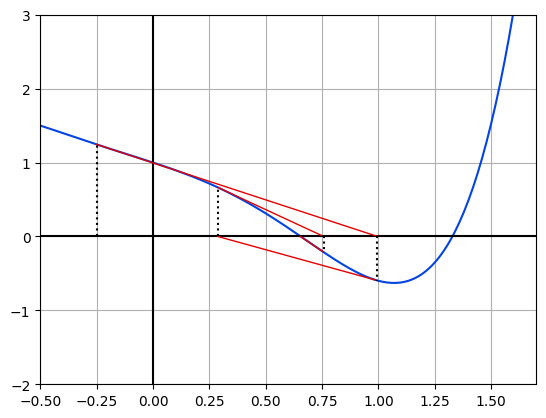
\includegraphics[width=0.6\linewidth]{addons/newton_method}
\end{center}

\section{Bootstrap}
\emph{Bootstrap} is an algorithm that allows to determine a vector of values that are implicitly defined by a set of equations.

Consider the following system 
\begin{equation}
	\begin{cases}
		f_1(x_1, c) = 0\\
		f_2(x_1, x_2, c) = 0\\
		f_3(x_1, x_2, x_3, c) = 0\\
		\vdots
		f_n(x_1,\ldots,x_n, c) = 0\\
	\end{cases}
\label{eq:bootstrap}
\end{equation}
It is possible to find the vector $\bar{x} = \{x_1,\ldots,x_n\}$ which simultaneously satisfy all the equation in~\ref{eq:bootstrap}, with an iterative algorithm as follows.
Indeed, solving the first equation, either analytically or numerically, we get $x_1 = f_1^{-1}(c)$ that can be used to solve the second equation as $x_2 = f_2^{-1}(x_1, c)$.
Going on, \emph{iteratively}, through each equation we are then able to determine all the unknown $\bar{X}$ values.

As a financial example, you can imagine the functions $f_i$ as the pricing equation of bonds with different maturities, each depending on a different set of interest rates, minus the current market price of the bond $c$. Since those are fair prices each $f_i$ can be set equal to 0 and through the bootstrap we can determine the interest rate term-structure implied by the bond market quotes. 

Another practical application of the bootstrap algorithm is to determine the \emph{spot cap volatilities} from the current market prices (note, the market quotes only the flat volatilities).
%The main challenges are:
%\begin{enumerate}
%		\item Produce Caplet/Floorlet prices consistent with current levels of Cap/Floor volatilities and therefore be able to re-price the market;
%	\item being able to “rebase” volatilities when pricing Cap/Floor over not quoted floating rates according to multiple curves framework (e.g. Cap/Floor over 1M or 12M Euribor);
%	\item to make things more complicated, some Caps/Floors are not always quoted over the same LIBOR, for example EUR Cap/Floor are quoted over 3M EURIBOR up to $2y$ maturity and then over 6M EURIBOR.
%\end{enumerate}

From the prices of different maturity caps, it is possible to \emph{bootstrap} the volatility of each caplet, i.e. the volatility which refers to the forward rate corresponding to the caplet.

\section{Negative Rates}

The financial crisis, which started in 2007, exposed a lack of trust among counterparties. Since then the incorporation of the probability of default in pricing models has become standard.
This lack of trust in the financial system reduced trading activities and kept the money in the pockets.
To recover trust, the central banks decide to intervene and stimulate the monetary supply and demand by lowering the interest rates.
This decision was expected to encourage investors to borrow money at low rate and invest into the economy, which would push its grow. Since 2008 interest rates have gradually been lowered.

Begin June 2014, the rates set by ECB were negative for the first time (-10 bps). Using negative rates to "inspire" investors is certainly unconventional bu not unprecedented (Switzerland, Sweden and Denmark also report negative rates).

In a negative interest rate environment, the ZCBs, may get values that are higher than one unit of currency. This would imply that the Libor rate would be negative. When the the rate is negative the Black-Scholes pricing equation is not properly defined (the logarithm of a negative quantity...).

Instead of using the Geometric Brownian Motion dynamics, the arithmetic Brownian Motion (ABM), that give rise to negative realizations could, for example be chosen. Such a solution, although straight-forward, has a significant disadvantage, however, as the normal distribution has much flatter tails as compared to a log-normal process. Figure\ref{fig:lognormal_shifted} shows the density of various log-normal  distributions. Notice how the bigger is the shift the wider is the distribution.

So instead of completely changing the underlying dynamics, the industrial standard fro dealing with the negativity has become to \emph{shift} the original process.

Caplets can be prices under a negative interest rate environment by an \emph{adaptation} of the underlying dynamics of the Libor rate. The shifted process is defined, as
\begin{equation}
\hat{L_k}(t) = L_k(t) + \theta_k
\end{equation}
The corresponding Black equation becomes
\begin{equation}
	\textbf{Cpl}_k(t_0) = N\tau_k P(t_0, T_k)\left[\hat{L_k}(t_0)\Phi(d_1)-\hat{K}\Phi(d_2)\right] 
\end{equation}
where $\hat{K} = K + \theta_k$.

\begin{figure}[htbp]
\begin{center}
	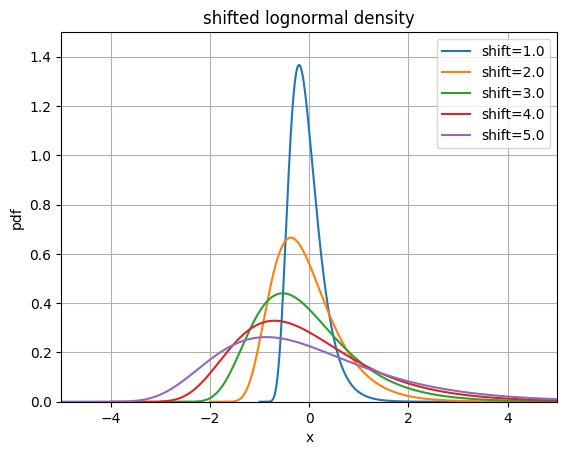
\includegraphics[width=0.6\linewidth]{addons/lognormal_shifted}
\end{center}
\caption{Density of various log-normal  distributions. Notice how the bigger is the shift the wider is the distribution.}
\label{fig:lognormal_shifted}
\end{figure}

%\section{Jamshidian Decomposition}
%An option on a portfolio of pure discount bonds can be decomposed into a portfolio of options on the individual discount bonds in the portfolio.
%
%Hence, we can think of the European Swaption as a sum of European
%options on Zero-Coupon bonds. This method is called Jamshidian’s decomposition, and is mathematically explained as follows:
%\begin{equation}
%	\max\left[\sum_{i=1}^n C_i p(r, t, s_i) - K, 0\right] = \sum_{i=1}^n C_i \max\left[p(r, t, s_i) - K_i, 0\right]
%	\label{eq:jamshidian_decomposition}
%\end{equation}
%
%Consider a European Swaption with strike rate $K$, maturity $T$ and nominal $FV$
%with payment dates $T_i$ for $i = 1,\ldots, n$. Since the value of a floating rate bond is worth its face value, we can take it as an option on a bond paying $C_i = K_{s_i}$ with strike price $FV$. This option will be exercised when $r(T) < r^*$ where $r^*$ is the solution to
%\begin{equation}
%	FV = \sum_{i=1}^n C_i p(r^*, T, T_i)
%\end{equation}
%This means that $FV$ is taken as a sum of discounted flows $C_i$ for a short rate $r^*$ at time $T$. To find the value of $r^*$ we have to discount all the Swap cash-flows, sum them up and let the sum be equal to the notional. We have to use the Newton-Raphson algorithm to follow this calculation $r^*$, that will be the correspondent level of $r$ for that equality to happen. 
%
%Once $r^*$ is found, we have to calculate the discounted cash-flows substituting it in the discounting factor $e^{-r\Delta t}$ and let them be the strike prices of our call options on Swaps.
%Afterwards, we calculate the payoff of the call options on the cash-flows with
%the strike price mentioned and sum them up. The payoff of this sum of options
%will thus be
%\begin{equation}
%	\max\left[\sum_{i=1}^n C_ip(r, T, T_i)-FV, 0\right]
%\end{equation}
%which using Eq.~\ref{eq:jamshidian_decomposition} we find is equivalent to
%\begin{equation}
%	\sum_{i=1}^n C_i \max\left[p(r, T, T_i)-FV_i, 0\right]
%\end{equation}
%where $FV_i = p(r^*, T, T_i)$. 
%Therefore, the Swaption is calculated as the sum of $n$ options on discounted bonds with the exercise price of the $i$th option equal to $FV_i$.
%
%After the price of a European Swaption under the Hull-White model is calculated, we have to calibrate it against the market data. Usually this calibration method is carried out taking the target prices to match the ones given by the Black-76 or Normal-Black models and trying to get as close as possible to them.

\section{Longstaff-Schwartz Algorithm}

Monte Carlo simulation is a flexible and powerful numerical method to value financial derivatives of any kind. However being a forward evolving technique, it is per se not suited to address the valuation of American or Bermudan options which are valued in general by backwards induction. Longstaff-Schwartz provide a numerically efficient method to resolve this problem by what they call \emph{Least-Squares Monte Carlo}.

The problem with Monte Carlo is that the decision to exercise an American option or not is dependent on the \emph{continuation} value. %Consider a simulation with $M+1$ points in time and paths. 
The approach of Longstaff-Schwartz approximates continuation values for American options in the backwards steps by an ordinary least-squares regression.
Equipped with such approximations, the option is exercised if the approximate continuation value is lower than the value of immediate exercise. Otherwise it is not exercised.

\subsection{Bermudan Option}
Consider a Bermudan put option with strike $K$ and maturity in $n$ years. Each year you can choose whether to exercise or not.
Let's implement a MC which actually simulates, besides the evolution of the market, what an investor holding this option would do. 

We simulate that 1 year has passed, computing the new value of the asset and of the money market account
\begin{equation}
	\begin{gathered}
		S(t_1=1y) = S(t_0)e^{(r-\frac{1}{2}\sigma^2)(t_1-t_0)+\sigma\sqrt{t_1-t_0}\mathcal{N}(0,1)} \\
		B(t_1=1y)=B(t_0)e^{r(t_1-t_0)}
	\end{gathered}
\end{equation}

At this point how does the investor know if it is convenient to exercise ? 
If it does he knows exactly the payoff he's getting. In case he continues, he knows that it is the same of having a European Put Option.

So, in mathematical terms we have the following payoff in 
\begin{equation}
	\max[K-S(t_1), P(t_1,T;S(t_1),K)]
\end{equation}
where $P(t_1,T;S(t_1),K)$ is the price of a Put which can be computed analytically! In the jargon of American products, 
is called the \emph{continuation value}, i.e. the value of holding the option instead of early exercising it.

The premium of the option is the average of this discounted payoff calculated in each iteration of the Monte Carlo procedure
\begin{equation}
	\cfrac{1}{N}\sum_i\max[K-S(t_1), P(t_1,T;S(t_1),K)]
\end{equation}

We could have priced this product because we have an analytical pricing formula for the put, but what if we didn't have it?

\textbf{Brute force solution}: for each realization of $S(t_1)$ we run another Monte Carlo to price the put. This method (called \emph{Nested Monte Carlo}) is very time consuming and quite inefficient. For this very simple case it's time of execution grows as $N^2$, which becomes prohibitive when you deal with more than one exercise date !

Let's search then for a finer solution analyzing the relationship between the continuation value and the simulated realization of $S$ at step $t_1$, by plotting the discounted payoff at maturity, $P_i$ vs $S_i(T_1)$ (the red line represents the analytical price of the put as a function of $S_i$), see Fig.~\ref{fig:continuation_function}.

%\begin{figure}[htbp]
%	\begin{center}
%		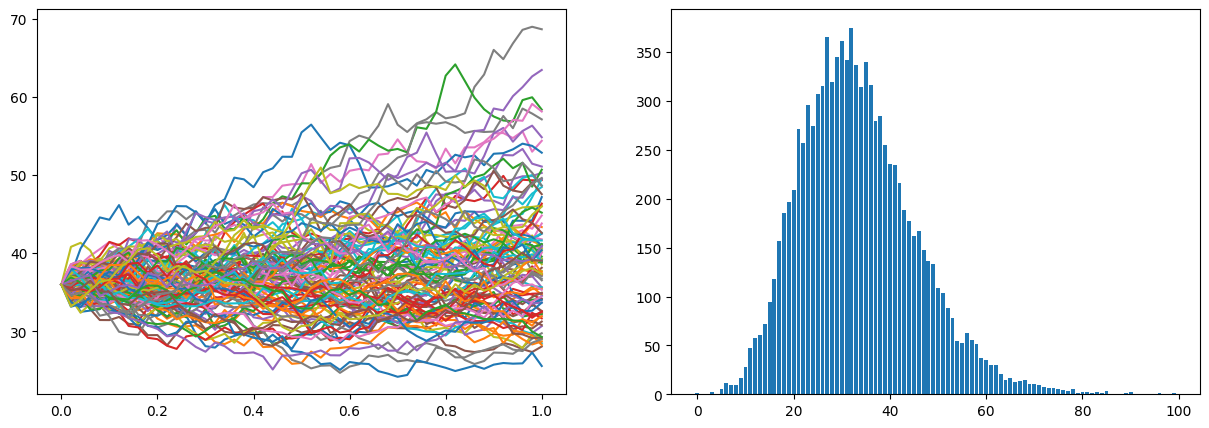
\includegraphics[width=0.8\linewidth]{addons/lsm_paths}
%	\end{center}
%	\label{fig:lsm_paths}
%\end{figure}

The analytical price of the put is a curve which kinds of interpolate the cloud of Monte Carlo points. This suggest us that
\textbf{the price at time $t_1$ can be computed by means of an average on all discounted payoff (i.e. the barycentre of the cloud made of discounted payoff)}.
Which in turn suggest that \textbf{the future value of an option can be seen as the problem of finding the curve that best fits the cloud of discounted payoff up to date of interest.}

As an example in Fig.~\ref{fig:continuation_function} there is a curve found by means of a linear regression on a polynomial of 5th order.

\begin{figure}[htbp]
	\begin{center}
		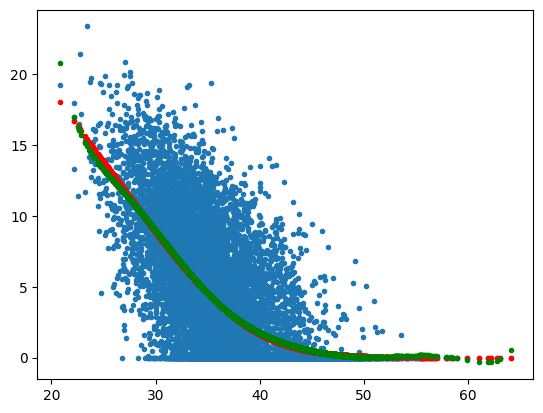
\includegraphics[width=0.5\linewidth]{addons/continuation_function}
	\end{center}
	\caption{Simulations of the continuation value for the option. The Black-Scholes price and the best fit of a $5^{th}$ order polynomial are also shown.}
	\label{fig:continuation_function}
\end{figure}

So we have an empirical pricing formula for the put to be used in the Monte Carlo Simulation
\begin{equation}
	P(t_1,T,S(t_1),K)=c_0+c_1 S(t_1) + c_2 S(t_1)^2 + c_3 S(t_1)^3 + c_4 S(t_1)^4 + c_5 S(t_1)^5
\end{equation}

The formula is obviously fast, the cost of the algorithm being just the best fit. Clearly we could have used any form for the curve (not only a polynomial). 

\subsection{The Algorithm}
The major insight of Longstaff-Schwartz is to estimate the continuation value $C_{t,i}$ by ordinary least-squares regression, therefore the name Least Square Monte Carlo for the algorithm. 
Their goal is to regress the $I$ continuation values $Y_{t,i}$ against the I simulated levels $S_{t,i}$. Given $D$ basis functions $b_i:\mathbb{R}^D\rightarrow\mathcal{R}$ for the regression, the continuation value $C_{t,i}$ is according to the approach approximated by
\begin{equation}
	\hat{C}_{t,i}=\sum_{i=1}^D \alpha^*_{d,t}b_d(S_{t,i})
	\label{eq:continuation_approx}
\end{equation}

The optimal regression parameters $\alpha^*_{d,t}$ are the result of the minimization
\begin{equation}
	\min_{\alpha_{1,t},\ldots,\alpha_{D,t}}\cfrac{1}{I}\sum_{i=1}^I \left(Y_{t,i}-\sum_{i=1}^D\alpha^*_{d,t}b_d(S_{t,i})\right)^2
	\label{eq:optimization_alphas}	
\end{equation}

In some circumstances, the quality of the regression can be improved upon when restricting the paths involved in the regression to those where the option is in-the-money.

Let's consider now a generic American product. Here is the Longstaff-Schwartz algorithm
\begin{itemize}
	\item simulate $I$ index level paths with $M+1$ points in time leading to index level values
	\begin{equation*}
		S_{t,i},\quad t \in \{0,\ldots,T\}, i \in \{1,\ldots,I\}
	\end{equation*};
	\item for $t=T$ the option value is $V_{T,i}=h_T(S_{T,i})$ by arbitrage arguments;
	\item start iterating backwards $t = T-\Delta t, \ldots,\Delta t$:
	\begin{itemize}
		\item regress the $T_{t,i}$ against the $S_{t,i}, i\in \{1,\ldots, I\}$, given $D$ basis function $b$;
		\item approximate $C_{t,i}$ by $\hat{C}_{t,i}$ according to Eq.~\ref{eq:continuation_approx} given the optimal parameters $\alpha^*_{d,t}$ from Eq.~\ref{eq:optimization_alphas};
		\item set 
		\begin{equation*}
			V_{t,i}=
			\begin{cases}
				h_t(S_{t,i})\quad\text{if }h_t(S_{t,i})>\hat{C}_{t,i}\text{ exercise takes place}\\
				Y_{t,i}\quad\text{if }h_t(S_{t,i})\leq\hat{C}_{t,i}\text{ exercise does not take place}\\
			\end{cases}
		\end{equation*}
		repeat iteration steps until $t=\Delta t$;
	\end{itemize} 
	\item for $t=0$ calculate the LSM esitmator
	\begin{equation}
		\hat{V}_0^{LSM}=e^{-r\Delta t}\cfrac{1}{I}\sum_{i=1}^{I}V_{\Delta t, i}
	\end{equation} 
\end{itemize}

In their paper, Francis Longstaff and Eduardo Schwartz found that using Laguerre, Hermite, Legendre or simple powers made very little difference in the results. 

There are indeed many more significant choices in the regression techniques:
\begin{itemize}
\item the overall power and the choice of variables (e.g. scaled variables);
\item include all paths or just the in-the-money paths;
\item regression technique (e.g. Cholesky, QR, SVD);
\item are polynomials a good choice at all ? Should you consider other kinds of regressions ?
\end{itemize}

Now, the choice of Laguerre polynomials may facilitate the regression result. Laguerre polynomials are orthogonal with regards to the exponential function. This emphasizes the data at a particular sample and de-emphasizes more distant data. It is possible that the resulting linear system is better behaved then. 

\section{Callable Bond}
A callable bond is a bond in which the issuer reserves the right to redeem the bond at different discrete times, possibly for different redemption values. When a callable bond is bought, no one knows when the bond will be called, however it can only be called at the times agreed upon at issue.

Investors have a variety of tools and techniques at their disposal, which enable them to assess the value of callable bonds and make informed investment decisions. Examples are:
\begin{itemize}
\item \textbf{Yield to Call (YTC)} It is a measure of the return an investor can expect if a callable bond is called by the issuer. It takes into account the call price, the coupon rate, and the time to call. YTC is an important metric for investors because it allows them to compare the potential return of a callable bond to that of a non-callable bond. However, it is important to note that YTC assumes that the issuer will call the bond at the first opportunity, which may not always be the case.
%\item \textbf{Yield to Worst (YTW)} It is a measure of the return an investor can expect if a callable bond is not called by the issuer. It takes into account the yield to maturity and the yield to call, whichever is lower. YTW is important for investors because it provides a more conservative estimate of the potential return of a callable bond. It is also important to note that YTW assumes that the bond will not be called, which may not always be the case.
%\item \textbf{Option-Adjusted spread (OAS)} It is a measure of the yield spread between a callable bond and a risk-free bond of the same maturity. It takes into account the optionality of the callable bond, which allows the issuer to call the bond at any time. OAS is important for investors because it provides a more accurate estimate of the credit risk associated with a callable bond.
\item \textbf{Duration} It is a measure of the sensitivity of a bond's price to changes in interest rates. It takes into account the bond's cash flows, maturity, and yield. Duration is important for investors because it allows them to assess the risk associated with a callable bond. Callable bonds typically have shorter durations than non-callable bonds, which means that they are less sensitive to changes in interest rates.
\item \textbf{Monte Carlo Simulation}.
\end{itemize}

The most common questions asked with callable bonds involve either determining the maximum price that can be paid for the bond to guarantee a certain yield rate, or detemining the minimum yield rate for a bond that was bought at a certain price.

The recommende strategy in both cases is to crete a sort of two column table with the first representing the time at which the bond can be called.

For the first type of problems, the second column is the corresponding price in order to receive the desired yield rate, \%, keeping in mind the redemption value may be different at the different redemption dates. Then think through what happens whine the bond is bought for the prices in the table but redeemed at other times in the table, an answer the question accrodgingly.
while for the second is the yield rate tha would produce the given price. \%, again keeping in mind the redemption value may be different at the different redemption dates.

\section*{Exercises}
\begin{exercise}[subtitle=Forward Rate Agreement]
A $3\times 9$ Forward Rate agreement refers to:
\begin{itemize}
\item a 90-day LIBOR loan starting 270 days from now;
\item a 270-day LIBOR loan starting 90 days from now;
\item a 180-day LIBOR loan starting 90 days from now.
\end{itemize}
\end{exercise}
\begin{solution}
The correct answer is (c). $3\times 9$ means a 180-day LIBOR loan starting 90 days from now.
\end{solution}

\begin{exercise}[subtitle=FRA Valuation]
Suppose we have a $1\times 4$ FRA with a notional principal of €1 million. 
At contract expiration, the 90-day LIBOR at settlement is 6\% and the contract rate is 5.5\%.
Calculate the value of the FRA at maturity.
\end{exercise}
\begin{solution}
Since the settlment rate is higher than the contract rate, the buyer will be receiving money from the seller. The payment at settlment is as follow:
$P = 1M\cdot(6\%-5.5\%)\cdot \cfrac{90}{360} = 1250$

Discounted back 90 days at 6\% gives
$P = \cfrac{1250}{1+\frac{90}{360}\cdot0.06} = 1231.53$
\end{solution}

\begin{exercise}[subtitle=Forward Rate Agreement]
The following term structure of LIBOR is given 
\begin{table}[htbp]
\begin{center}
\begin{tabular}{c|c}
90 days & 6.00\% \\ \hline
180 days & 6.20\% \\ \hline
270 days & 6.30\% \\ \hline
360 days & 6.35\% \\
\end{tabular}
\end{center}
\end{table}
\begin{itemize}
\item Find the rate on a new 6 × 9 FRA;
\item Consider an FRA that was established previously at a rate of 5.2 percent with a notional amount of 30~M. The FRA expires in 180 days, and the underlying is 180-day LIBOR. Find the value of the FRA from the perspective of the party paying fixed and receiving floating as of the point in time at which this term structure applies.
\end{itemize}
\end{exercise}
\begin{solution}
\begin{itemize}
\item The contract at inception has to be "fair" so the requested rate is the break-even rate of the contract or the forward rate $F(t; T=180, S=270)$, hence
\begin{equation*}
K = \cfrac{6.3\cdot\frac{9}{12}-6.2\cdot0.5}{\frac{9}{12}-0.5} = 6.5\%
\end{equation*}
\item The old contract value (seen by the party paying fixed) is given by 
\begin{equation*}
\textbf{FRA} = -N\cdot[P(t,S)\tau K - P(t,T) + P(t, S)]
\end{equation*}
where $t=T=0$, so $P(0,S)=e^{-0.062*0.5}= 0.9695$, $\tau=0.5$ and $P(t,T)=1$.
\begin{equation*}
\textbf{FRA} = 237279
\end{equation*}
a positive value was expected since $K<L$.
\end{itemize}
\end{solution}

\begin{exercise}[subtitle=Forward Rate]
The 1-year spot rate on US treasury bonds is 9\%, the 2-year spot rate is 9.5\% and the 3-year spot rate is 10\%. 
\begin{itemize}
\item Calculate the implied 1-year ahead, 1-year forward rate, $F(0;1,2)$. Explain why a 1-year forward rate of 9.6\% could not be explained by the market;
\item calculate the forward rates  $F(0; 2, 3$ and $F(0; 1,3)$. Is there a link between $F(0;1,2),F(0;2,3)$ and $F(0;1,3)$ ?
\end{itemize}
\end{exercise}
\begin{solution}
\begin{itemize}
\item The forward rates are as follows:
\begin{equation}
\begin{aligned}
F(0;1,2) &= \cfrac{0.095*2 - 0.09*1}{2-1} = 0.1, \quad F(0;2,3)= \cfrac{0.1*3 - 0.095*2}{3-2} = 0.11, \\ 
F(0;1,3) &= \cfrac{0.1*3 - 0.09*1}{3-1} = 0.105
\end{aligned}
\end{equation}
If you lend €100 at $t=1$ at 9.6\%, your cash flow is -€100 at $t=1$ and €109.6 at $t=2$. 

You can do better by borrowing now for 1 year $€100/1.09=€91.74$ and lending the same amount for 2 years. Your net cash flow is then €0 at $t=0$, -€100 at $t=1$ (that is $€91.74\cdot 1.09$), and €110 at $t=2$ (that is $€91.74\cdot 1.095^2$). 

Compared to the first option, you have thus a certain higher cash flow at $t=2$: €110 vs. €109.6.  There is no reason to accept the 9.6\% rate contract. 
\item The link between the forward rate is as follows:
\begin{equation}
\cfrac{(1+F(0;1,3))^2}{1+F(0;1,2)} = \cfrac{(1+r_3)^3}{(1+r^2)} \Rightarrow (1+F(0;1,3)^2 = (1+F(0;1,2))(1+F(0;2,3))
\end{equation}
Hence, with any two of three forward rates, you can deduct the third one.
\end{itemize}
\end{solution}

\begin{exercise}[subtitle=Forward Rate]
A bank offers to borrow €100 from you at an interest rate applicable between the end of year 1 and the end of year 2 at a rate of 13\% (i.e. the forward rate). The spot rates for 1-year and 2-year are currently 10\% and 12\% respectively. Explain whether you would take the bank’s offer. 
\end{exercise}
\begin{solution}
The forward rate between year 1 and year 2 is $F(0;1,2)=14\%$. It can be shown that it is irrational to accept lending at 13\% at year 1. 

Indeed, if you lend €100 at $t=1$ at 13\%, your cash flow is -€100 at $t=1$ and €113 at $t=2$.
 
You can do better by borrowing now for 1 year $€100/1.10=€90.91$ and lend the same amount for 2 years. Your net cash flow is then €0 at $t=0$, -€100 at $t=1$ ($€90.91\cdot 1.10$), and €114.04 at $t=2$ (that is $90.91\cdot 1.12^2$). 

Compared to the first option, you have thus a certain higher cash flow at $t=2$: 114 vs. 113.  There is then no reason for the lender to accept the 13\% rate contract. 
\end{solution}

\begin{exercise}[subtitle=IRS as FRA sum (\texttt{python})]
Implementing a \texttt{python} class or a function that represents an interest rate swap shows that:
\begin{enumerate}
\item in a \emph{Payer Swap} with an increasing yield curve the first FRAs will have negative value, the last positive;
\item in a \emph{Payer Swap} with a decreasing yield curve the first FRAs will have positive value, the last negative.
\end{enumerate}
\end{exercise}

\begin{exercise}[subtitle=Interest Rate Swap]
A 100~M interest rate swap has a remaining life of 10 months. Under the terms of the swap; 6-month LIBOR is exchanged for 7\% p.a. (compounded semiannually). The average of the bid-offer rate being exchanged for 6-month LIBOR in swaps of all maturities is currently 5\% p.a. with continuous compounding. The 6-month LIBOR rate was 4.6\% p.a. 2 months ago. 
\begin{itemize}
\item What is the current value of the swap to the party paying floating ?
\item What is its value to the party paying fixed ?
\end{itemize}
\end{exercise}
\begin{solution}
In four months 6~M ($0.5\times 0.12\times 100$~M) will be received and 4.8~M ($0.5\times 0.096\times 100$~M) will be paid. (We ignore day count issues.) In 10 months 6~M will be received, and the LIBOR rate prevailing in four months-time will be paid. The value of the fixed-rate bond underlying the swap is
\begin{equation*}
6 \exp(-0.1 \times 4/12) + 6 \exp(0.1\times  10/12) = 103.328\text{~M}
\end{equation*}
The value of the floating-rate bond underlying the swap is 
\begin{equation*}
(100 + 4:8) \exp(0.1\times  4/12) = 101364 \text{~M}
\end{equation*}
The value of the swap to the party paying floating is $103328-  101364 = 1964$~M. 
The value of the swap to the party paying fixed is the opposite. 

These results can also be derived by decomposing the swap into forward contracts. Consider the party paying floating. The first forward contract involves paying 4.8~M and receiving 6~M in four months. It has a value of $1.2e^{-0.1\cdot 4/12} = 1.161$~M.
To value the second forward contract, we note that the forward interest rate is 10\% per annum with continuous compounding, or 10.254\% per annum with semiannual compounding. The value of the forward contract is
\begin{equation*}
100\times  (0.12\times 0.5-0.10254\times 0.5)e^{-0.1\cdot 10/12} = 0.803 \text{~M}
\end{equation*}

The total value of the forward contract is therefore $1.161 + 0.803 = 1.964$~M.
\end{solution}

\begin{exercise}[subtitle=Interest Rate Swap]
Assume that company A has agreed to pay a 6-month Libor and receive a fixed interest rate of 8\% per annum (with interest payable every six months) from the face value of 100~M. Swap is 1.25 years to expire. The interest rates for 3, 9 and 15 months are: 10\%, 10.5\% and 11\% respectively. Assume that interest rates are continously compounded. The 6-month Libor is currently 10.2\%. Calculate the value of this swap for company A.
\end{exercise}
\begin{solution}
In our case: $Q= 100$~M - the principal of the swap (in bond notation it is face value FV), LIBOR=0.102 - 6 months LIBOR, T=1.25 - the maturity of the bond as a fraction of the year (15 months is 1.25 of year), r3m=0.10 - 3 months interest rate, r9m=0.105 - 9 months interest rate, r15m=0.11 - 15 months interest rate, rfix=0.08 - fixed interest rate, 2 - number of payments in a year

Since the company A pays floating interest and receives fixed one
\begin{equation*}
V=V_{fix}-V_{fl} = \sum_{i=1}^n \cfrac{k}{e^{r_i t_i}} + \cfrac{Q}{e^{r_n t_n}} - \cfrac{k^*}{e^{r_1 t_1}}+\cfrac{Q}{e^{r_1 t_1}}
\end{equation*}

The fixed leg value is
\begin{equation*}
V_{fix} = 4e^{-0.25\cdot 0.1} +  4e^{-0.75\cdot 0.105} +  104e^{-1.25\cdot 0.11} = 98.25\text{~M}
\end{equation*}

The floating payment is based on LIBOR and the nearest (first) payment is 
\begin{equation*}
k^*=0.102\cdot0.5\cdot 100 = 5.1\text{~M}
\end{equation*}
Hence:
\begin{equation*}
V_{fl}=5.1e^{-0.25\cdot 0.1}+100\cdot e^{-0.25\cdot 0.1} = 102.51
\end{equation*}

And the final calcualtion
\begin{equation*}
V = 98.24-102.51=-4.27\text{~M}
\end{equation*}
which is the swap value for company A.
\end{solution}

\begin{exercise}[subtitle=Interest Rate Swap]
Determine the value of the swap from previous exercise in the way as described in the Relationship between interest rate swap and FRA part.
\end{exercise}
\begin{solution}
The cash flows that will be exchanged after three months can be calculated at the beginning. The interest rate of 8\% will be exchanged for a rate of 10.2\%. Let us call it FRA1:
\begin{equation*}
FRA_1 = 0.5\cdot 100\cdot (0.08-0.102)\cdot e^{-0.25\cdot 0.1}=-1.07
\end{equation*}

Determination of flows after 9th and 15th month requires two more formulas.

First we have to calculate forward interest rate for the half-year period for 3 months from now. This is required to calculate the cash flow after 9 months. We will use the following formula: $e^{r_{9m}\cdot0.75}=e^{r_{3m}\cdot0.25}e^{F'_{0.25, 0.5}\cdot 0.5}$. Solving the formula for $F'_{0.25, 0.5}$ we have:
\begin{equation*}
F'_{0.25, 0.5}=\cfrac{r_{9m}\cdot 0.75-r_{3m}\cdot0.25}{0.5}=0.10750
\end{equation*}

The rate is continuously compounded therefore we should convert it into semi-annual compounding with the formula $R_m = m\cdot(e^{r_c/m}-1)$, where $r_c$ is continuously compounded and $r_m$ is discretely compounded. Note that $m$ in this formula is the number of payments within a year (not the number of months).
\begin{equation*}
F_{0.25, 0.5}=2\cdot(e^{F'_{0.25,0.5}/2}-1)=0.11044
\end{equation*}
The present value of the cash flow exchanged in 9 months is:
\begin{equation*}
FRA_2=0.5\cdot100\cdot(0.08-0.11044)\cdot e^{-0.75\cdot0.105}=-1.41
\end{equation*}
obtained from the FRA contract valuation.

Then the procedure goes on similarly: to calculate the present value of the cash flow that will occur in 1 year and 3 months, we need to calculate forward interest rate for the half-year period for 9 months from now. We will use the following formula: $e^{r_{15m}\cdot 1.25}=e^{r_{9m}\cdot 0.75}e^{F'_{0.75, 0.5}\cdot 0.5}$. Solving the formula for $F'_{0.75, 0.5}$
 we have:
\begin{equation*}
F'_{0.75, 0.5}=\cfrac{r_{15m}\cdot1.25-r_{9m}0.75}{0.5}=0.11750
\end{equation*}

After converting the rate with continuous compounding to the interest rate with semi-annual compounding, we obtain:
\begin{equation*}
FRA_{0.75,0.5}=2\cdot(e^{F'_{0.75,0.52}}-1)=2\dot(e^0.117502-1)=0.12102
\end{equation*}

The present value of the cash flow exchanged in 15 months is:
\begin{equation*}
FRA_3=0.5\cdot100\cdot(0.08-0.12102)\cdot e^{-1.25\cdot0.11}=-1.79
\end{equation*}

The value of the swap is then 
\begin{equation*}
V=FRA_1+FRA_2+FRA_3 = -1.07-1.41-1.79=-4.27
\end{equation*}
\end{solution}

\begin{exercise}[subtitle=FRN resetting (\texttt{python})]
Draw a plot showing the characteristic sawtooth behaviour of a floating rate note. The relevant insterest rates can be taken from \href{https://raw.githubusercontent.com/matteosan1/advanced\_financial\_modeling/master/input_files/libor.csv}{libor.csv}
\end{exercise}

\begin{exercise}[subtitle=Asset Swap Spread]
Consider the 10-year German bund DBR 0.5\% which is currently trading at a price of 104.58. Given that the 10-year swap rate is 0.44\% what is the par-par asser swap spread for this bond ? 
Then consider the corresponding 10-year Greek Governament Bond GGB 3.0\% which is currently trading at a price of 75.28. What is the par-par asset swap spread in this case ?
(Assume that the annuity factor have a value of 10 for simplicity).
\end{exercise}
\begin{solution}
\begin{equation*}
s_{DBR} = \cfrac{\frac{100-104.58}{100}}{10} = -46 bps
\end{equation*}
\begin{equation*}
s_{GGB} = \cfrac{\frac{100-75.28}{100}}{10} = 2.47\%
\end{equation*}
\end{solution}

\begin{exercise}[subtitle=Asset Swap]
Describe the asset swap contract for a coupon bond with coupons equal to $C$ and price equal to $P(t)$. 
What will happen to the price if the spread increase, all the rest being equal ?
What does it mean in term of credit quality epectation by the market for the bond's issuer ?
\end{exercise}

\begin{exercise}[subtitle=Asset Swap vs CDS (\texttt{python})]
Consider a 1Y risky bond paying quarterly coupons. The bond issuer has a default probability of 5\% during the next year. The interest rate term structure is considered flat at 0.05.

\begin{itemize}
\item If the bond buyer enters into an asset swap, determine its spread;
\item check that a CDS with same maturity as the asset swap has similar spread;
\item finally check how the spread change as a function of the probability of default.
\end{itemize}
\end{exercise}

\begin{exercise}[subtitle=DV01]
Consider a 2-year Interest Rate Swap on a notional of 1M, with a fixed rate of 5\% and paying Libor rate annually. The term-structure of interest rates is flat at 5\%.
Estimate the DV01 of the swap numerically.  
\end{exercise}
\begin{solution}
The DV01 can be approximated in two ways:
\begin{itemize}
\item $DV01 = \frac{\Delta P(+\delta r)-\Delta P(-\delta r)}{2}$ with $\delta r = 1 bps$
\begin{equation*}
DV01 = \cfrac{A(S+\delta r-K) - A(S-\delta r-K)}{2} = A\delta r = (e^{-0.05}+e^{-0.1})\cdot 0.0001 \approx 0.0002
\end{equation*}
\item $DV01 = 100\Delta P(\frac{1}{100}bps)$
\begin{equation*}
DV01 = 100\cfrac{A(S+ 10^{-6}-K) - A(S-K)}{2} = A 10^{-4} = (e^{-0.05}+e^{-0.1})\cdot10^{-4} \approx 0.0002
\end{equation*}
\end{itemize}
\end{solution}

\begin{exercise}[subtitle=AD for a Simple Function (\texttt{python})]
Consider the function defined in Eq.~\ref{eq:aad_function} and compute the AD both using tangent and adjoint technique.
\end{exercise}

\begin{solution}
\begin{equation}
\begin{cases}
\text{Function: } f(x_1, x_2) = 2x_1^2 + 3x_2\\
\text{Solution: } \frac{df}{dx_1} = 4x_1, \text{ and } \frac{df}{dx_2}=3
\end{cases}
\end{equation}
When for example $x_1=2$ and $x_2 = 3$ we have,
\begin{equation}
\frac{df}{dx_1} = 8, \text{ and } \frac{df}{dx_2}=3
\end{equation}
\end{solution}

\begin{exercise}[subtitle=AD for a Swap (\texttt{python})]
Consider a 5-years receiver Interest Rate Swap with a 1M notional, exchanging a fixed rate of 5\% with a flat 1\% LIBOR rate, with annual payments. 
Compute DV01 and PV01 with algorithmic differentiation using both tangent and adjoint modes. Compare the results.
\end{exercise}

\begin{exercise}[subtitle=BS Implied Volatility (\texttt{python})]
Consider a European call option with the following parameters: $S_0=30$, $K=28$, $T=3m$, $r=0025$ and $\sigma=0.3$.
%market_price = 3.9790765403377035

Using the Newton-Raphson method determined the implied volatility.
\end{exercise}

\begin{exercise}[subtitle=Shifted Brownian Motion (\texttt{python})]
Write a python function that simulated shifted-geometric Brownian motion paths.
\end{exercise}

\begin{exercise}[subtitle=Negative Rates (\texttt{python})]
Using the function written in the previous exercise, price caplets with Monte Carlo and using Black formula in a regime with negative interest rates. Compare the two results.
\end{exercise}

\begin{exercise}[subtitle=Cap Volatilities (\texttt{python})]
Given the following set of flat volatilities use the bootstrap algorithm to determine the implied spot volatilities.

Let's \emph{strip} caplet volatilities from the following cap (flat) volatilities which refers to caps with 0.013 strike over EURIBOR-6M whose term structure is shown in Table~\ref{tab:flat_volatilities}(right).

\begin{table}[htpb]
\begin{center}
\renewcommand{\arraystretch}{2}
\begin{tabular}{|c|c|}
\hline
Maturity & Volatility \\ \hline
1y & 44\% \\ \hline
2y & 45\% \\ \hline
3y & 44\% \\ \hline
4y & 41\% \\ \hline
5y & 39\% \\ \hline
\end{tabular}
\quad
\begin{tabular}{|c|c|}
\hline
Pillar & Rate \\ \hline
3m & 0.0002 \\ \hline
6m & 0.0007 \\ \hline
12m & 0.0025 \\ \hline
2y  & 0.0070 \\ \hline
3y & 0.0100 \\ \hline
5y & 0.0162 \\ \hline
\end{tabular}
\end{center}
\label{tab:flat_volatilities}
\caption{Left, flat volatilities table. Right, term structure of the considered Euribor-6M curve.}
\end{table}
\end{exercise}

\begin{exercise}[subtitle=Jamshidian Trick (\texttt{python})]
Consider the process 
\begin{equation*}
\psi_i(X)=e^{-t_i}|X|,\quad t_i=\{0,1,2,\ldots, N\}
\end{equation*}
with $X\approx\mathcal{N}(0,1)$.

Compute 
\begin{equation*}
A = \mathbb{E}\left[\max\left(\sum_{k=1}^N \psi_k(X) - K, 0\right)\right]
\end{equation*}
both directly using Monte Carlo simulation and by using Jamshidian's decomposition.
Plot the results against the strike $K$.
\end{exercise}

\begin{exercise}[subtitle=Jamshidian Trick (\texttt{python})]
Implement the Jamshidian decomposition to price swaptions under the Vasicek short rate model.
\end{exercise}

\begin{exercise}[subtitle=Longstaff and Schwartz (\texttt{python})]
Price an Bermudan Swaption using the Longstaff-Schwartz algorithm. %The initial underlying value is $S_0=36$, the volatility is 20\%, the strike price $K=40$, $T=1$, and the risk-free rate 6\% flat.
\end{exercise}

\begin{exercise}[subtitle=Longstaff and Schwartz (\texttt{python})]
Price an American put option using the Longstaff-Schwartz algorithm. The initial underlying value is $S_0=36$, the volatility is 20\%, the strike price $K=40$, $T=1$, and the risk-free rate 6\% flat.	
\end{exercise}

\begin{exercise}[subtitle=Callable Bond (\texttt{python})]
A 1000 face value 20-years callable bond with 5\% annual coupons is selling 1150. The bond can be redeemed at the end of 18 years for 950, at the end of 19 years for 975, or at the end of 20 years for 1000. Determine the minimum annual yield rate that a buyer will earn on this bond.
\end{exercise}

\begin{exercise}[subtitle=Callable Bond (\texttt{python})]
A 1000 face value 20-year callable bond with 3\% annual coupons can be redeemed according to the following schedule:
\begin{itemize}
	\item 1000 at the end of years 10 through 14;
	\item 1075 at the end of years 15 through 17;
	\item 1125 at the end of years 18 through 20.
\end{itemize}
Determine the maximum price a buyer should pay in order to earn an annual yield of at least 5\%.
\end{exercise}

%\begin{exercise}[subtitle=Callable Bond (\texttt{python})] 
%A 1000 face value 10-year callable bond with 8\% semiannual coupons is bought for 1050.  The bond can be redeemed at the end of any year starting with year 7.  Determine the minimum annual yield for this bond.
%\end{exercise}
%
%\begin{exercise}[subtitle=Callable Bond (\texttt{python})]
% A 1000 face value 20-years callable bong, reddeemable at 1200, with 5\% annual coupons can be redeemed at the end of year 18, 19, 20. Determine the maximum price a buyer is willing to pay in order to earn an annual yield of at least 3\%
%\end{exercise}
%
%\begin{exercise} A 1000 face value 20-years callable bond with 4\% annual coupons can be redeemed according to the following schedule:
%1000 at end 12-14, 1025 at end 15-17, 975 at end 18-20.
%Determine the maximum price a buyer is willing to pay in order to earn an annual yield of at least 4\%
%987.66
%\end{exercise}
%
%\begin{exercise} A 1000 face value 10\% annual coupon bond is redeemable as follows: 1100 at 15, 16,17, 1000 at 18,19,20. A buyer pays 1500 for this bond, Determine the buyer minimum annual yield.
%\end{exercise}
%
%\begin{exercise} A 20-year 10\% 1000 bond that pays interest half-yearly is redeemable (callable) in twelve years at a buy-back (call) price of 1150. The bond's current yield to maturity is 9.50\% annually. You are required to determine 
%\begin{enumerate}[label=(\alph*),font=\itshape]
%	\item the yield to call;
%	\item the yield to call if the buy-back price is only 1100;
%	\item the yield to call if instead of twelve years the bond can be called in eight years, the buy-back price being 1150.
%\end{enumerate}
%\end{exercise}

\begin{exercise}[subtitle=To Exercise or Not To Exercise (\texttt{python})]
Determine the interest rate value threshold that suggest an issuer to exercise a callable bond.
\end{exercise}

\begin{exercise}[subtitle=Vega]
Calculate the analytical expressions for:
\begin{itemize}
\item Delta Sensitivity analytically, that is the first derivative of caplet price w.r.t. the forward rate, using the black model to price a generic caplet;
\item Delta Vega analytically, that is the first derivative of caplet price w.r.t. the volatility, using the black model to price a generic caplet.
\end{itemize}
\end{exercise}

\begin{solution}
The Black formula for a caplet is given by:
\begin{equation*}
\textbf{Cpl} = L\delta_k P(0,t_{k+1})[F_k N(d_1)-R_k N(d_2)]
\end{equation*}
where:
\begin{equation*}
d_1 =\cfrac{\ln(F_k/R_k)+\sigma^2_k t_k/2}{\sigma_k \sqrt{t_k}},\text{ and } d_2 = d_1-\sigma_k \sqrt{t_k}
\end{equation*}

The delta will just be the first derivative of the equation above in respect to $F$, although one also has to worry about the $F$ being in the $d_1$ and $d_2$ terms.

Ignoring the constants $L\delta_k P(0,t_{k+1})$
\begin{equation*}
\Delta =\cfrac{\partial C}{\partial F} = N(d_1) + F\cfrac{\partial N(d_1)}{\partial F} - r_k\cfrac{\partial N(d_2)}{\partial F}
\end{equation*}
Next we apply the chain rule:
\begin{equation*}
	\cfrac{\partial N(d_1)}{\partial F} = \cfrac{\partial N(d_1)}{\partial d_1}\cfrac{\partial d_1}{\partial F}
\end{equation*}
and so:
\begin{equation*}
\Delta = N(d_1) + F\cfrac{\partial N(d_1)}{\partial d_1}\cfrac{\partial d_1}{\partial F} - R_k \cfrac{\partial N(d_2)}{\partial d_2}\cfrac{\partial d_2}{\partial F}
\end{equation*}
First thing to notice is that since the $d_1$ and $d_2$ definitions:
\begin{equation*}
\cfrac{\partial d_1}{\partial F} = \cfrac{\partial d_2}{\partial F}=\cfrac{1}{F_k\sigma_k\sqrt{t_k}}
\end{equation*}
and so:
\begin{equation*}
\Delta = N(d_1) + \cfrac{1}{F_k\sigma_k\sqrt{t_k}}\left[F\cfrac{\partial N(d_1)}{\partial d_1} - R_k \cfrac{\partial N(d_2)}{\partial d_2}\right]
\end{equation*}
Second, lets see how we can simplify the expression inside the parenthesis. Considering that:
\begin{equation*}
N(d_1) = \cfrac{1}{\sqrt{2\pi}}\int_{-\infty}^{d_1} e^{-x^2/2}dx
\end{equation*}	
it follows that:
\begin{equation*}
\cfrac{\partial N(d_1)}{\partial d_1}=N'(d_1)=\cfrac{1}{\sqrt{2\pi}}e^{-d_1^2/2}
\end{equation*}
and so:
\begin{equation*}
\left[F\cfrac{\partial N(d_1)}{\partial d_1} - R_k \cfrac{\partial N(d_2)}{\partial d_2}\right] = \left[FN'(d_1)-R_kN'(d_2)\right]
\end{equation*}

Now with a substitution of $d_2$ for $d_1-\sigma_k\sqrt{t_k}$, we have:
\begin{equation*}
\begin{gathered}
R_kN'(d_1 - \sigma_k\sqrt{t_k}) = R_k\cfrac{1}{\sqrt{2\pi}}\exp\left(\cfrac{-(d_1-\sigma_k\sqrt{t_k}))^2}{2}\right) = \\
= R_k\cfrac{1}{\sqrt{2\pi}}\exp\left(\cfrac{-d_1^2}{2}\right)\exp\left(\cfrac{-2d_1\sigma_k\sqrt{t_k}-(\sigma_k\sqrt{t_k})^2}{2}\right) = \\  = R_kN'(d_1)\exp\left(\cfrac{\ln(F_k/R_k)+\sigma_k^2t_k}{\sigma_k\sqrt{t_k}}\sigma_k\sqrt{t_k}\right)\exp\left(\cfrac{-\sigma_k^2t_k}{2}\right) = \\
=R_kN'(d_1)\exp\left(\ln(F_k/R_k)+\sigma^2_kt_k/2-\sigma^2_kt_k/2\right) = R_kN'(d_1)\cfrac{F_k}{R_k} = F_kN'(d_1)
\end{gathered}
\end{equation*}
and so
\begin{equation*}
	R_kN'(d_2)=F_kN'(d_1)
\end{equation*}
So finally, the delta of the caplet would be:
\begin{equation*}
\Delta = N(d_1) + \cfrac{1}{F_k\sigma_k\sqrt{t_k}}\left[FN'(d_1)-R_kN'(d_2)\right] =
N(d_1)
\end{equation*}
\end{solution}

%\begin{figure}[htbp]
%	\begin{center}
%		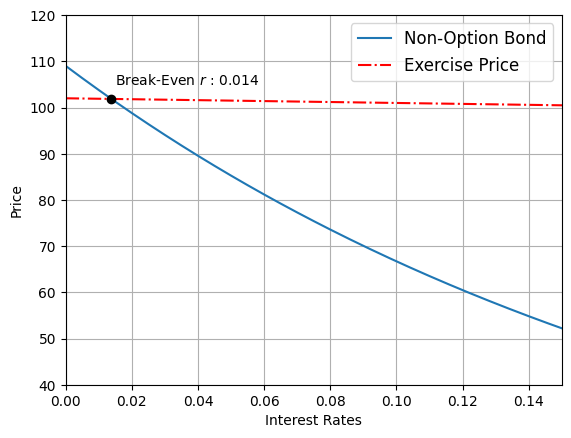
\includegraphics[width=0.5\linewidth]{addons/callable_bond}
%	\end{center}
%	\label{fig:callable_bond}
%\end{figure}

%\clearpage
%\section{Reverse Floater}
%
%* For instance, in September 2009, the short-term interest rate, the 3-month EURIBOR, **was at 0.5%**, and the forward curve was rising rather steeply, i.e. the implied forward 3-month EURIBOR in 3 years **was at 3.3%**. 
%* The 3-year interest rate for a fixed-coupon bond **was at 3.5%** at the time. 
%* It was possible to construct a 3-year reverse floater bond paying:
%
%$$ 6\% - 2 \cdot \text{3M-EURIBOR}$$
%
%(the coupon payments usually occur on a quarterly basis). 
%* Should the 3-Month EURIBOR not move during the first year, the coupon would amount to $6\% - 2 \cdot 0.5\% = 5\%$. 
%* Compared to a floating rate bond, the outperformance would be 4.5% for that period. 
%%* After 3 years, the invested nominal is redeemed along with the last coupon.
%
%Vega 
%
%$$V_{\text{cap}}=F\Phi(d_1) - K\Phi(d_2)$$
%
%$$\nu = \frac{\partial V_{\text{cap}}}{\partial\sigma} =
%F\phi(d_1)$$
%
%\begin{figure}[htbp]
%	\begin{center}
%		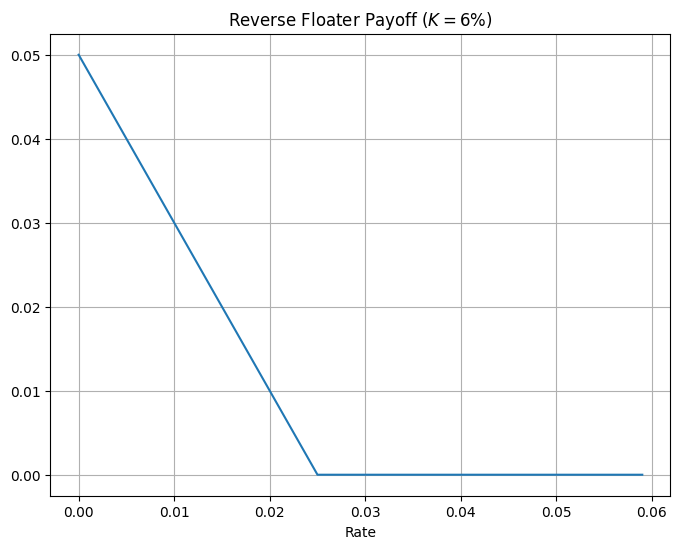
\includegraphics[width=0.5\linewidth]{addons/reverse_floater_payoff}
%	\end{center}
%	\label{fig:reverse_floater_payoff}
%\end{figure}
%
%\begin{figure}[htbp]
%	\begin{center}
%		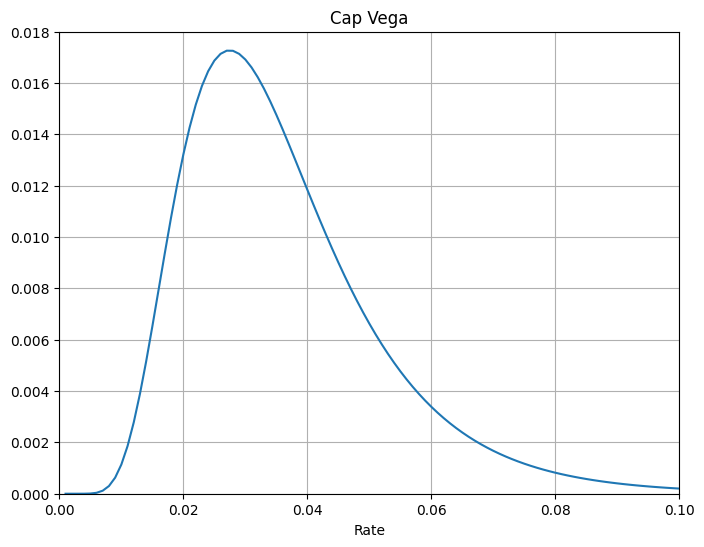
\includegraphics[width=0.5\linewidth]{addons/cap_vega}
%	\end{center}
%	\label{fig:cap_vega}
%\end{figure}

\chapter{Change of Measure}
\section*{Exercises}
%\begin{exercise}[subtitle=Drifty Brownian Motion]
%Let’s start with a standard Brownian motion $W_t^{\mathbb{P}} = \mathcal{N}_{\mathbb{P}}(0,t)$ under a probability measure $\mathbb{P}$, and adapted to a filtration $\mathcal{F}_t$. In Fig.~\ref{fig:brownian_motion_nodrift} 30 simulated path evolutions of $W_t^{\mathbb{P}}$ are shown, as expected there is no drift.
%	
%\begin{figure}[htbp]
%	\begin{center}
%		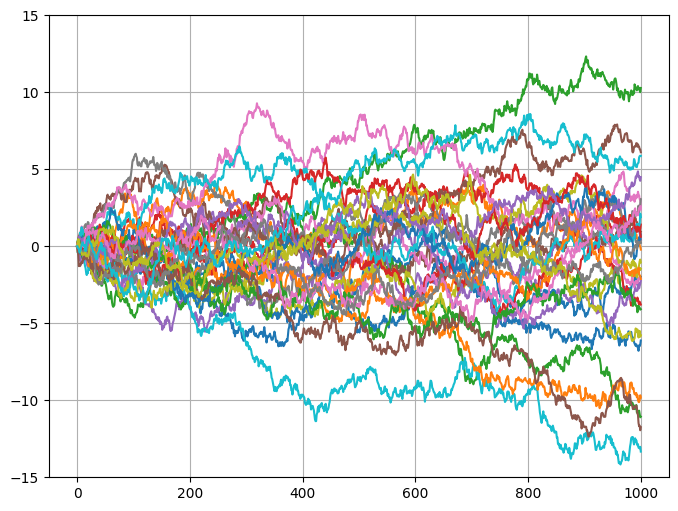
\includegraphics[width=0.5\linewidth]{addons/brownian_motion_nodrift}
%	\end{center}
%	\label{fig:brownian_motion_nodrift}
%	\caption{Thirty realization of the simple Brownian motion $W_t^{\mathcal{P}}$.}
%\end{figure}
%
%For exemplification, let us now construct a "drifty" process $Y_t=\mu t+\sigma W_t^{\mathcal{P}}\in \mathcal{N}_{\mathcal{P}}(\mu t, \sigma^2 t)$, that is a Wiener process with drift $\mu$ and diffusion $\sigma$; in other words, $\mathbb{E}^{\mathcal{P}}[Y_t]=\mu t$ and $\text{Var}^{\mathbb{P}}[Y_t]=\mathbb{E}^{\mathcal{P}}[Y^2_t]-\mathbb{E}^{\mathcal{P}}[Y_t]^2=\sigma^2 t$.
%
%%Incidentally, note the terminology: the drift is not an expectation, but rather the rate of change in expectation, and the diffusion is not a standard deviation, but rather the square root of the rate of change in variance. 
%Figure~\ref{fig:brownian_motion_drift} shows 30 simulated paths for the evolution of $Y_t$ ($\mu = 0.8$ and $\sigma =1.25$). There the drift is visually apparent.
%\begin{figure}[htbp]
%\begin{center}
%	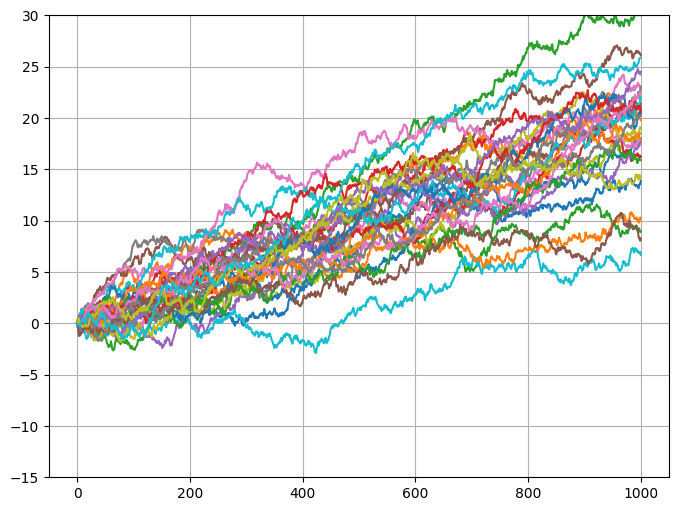
\includegraphics[width=0.5\linewidth]{addons/brownian_motion_drift}
%\end{center}
%\label{fig:brownian_motion_drift}
%	\caption{Thirty realization of the "drifty" Brownian motion $Y_t$.}
%\end{figure}
%
%We aim at applying a change of measure from $\mathcal{P}$ into a new probability $\mathcal{Q}$, such that $Y_t$ becomes driftless (a martingale) under $\mathcal{Q}: \mathbb{E}^{\mathcal{Q}}[Y_t]=0$, yet with the same diffusion as under $\mathcal{P}$: $\text{Var}^{\mathcal{Q}}[Y_t]=\sigma^2 t$
%
%Let $\mu^{*}$ be a new drift and assume $\\gamma_t = \frac{\mu_t^{*}-\mu_t}{\sigma_t}$. According to the Girsanov Theorem the process
%\begin{equation}
%dW^{*}_t = -\gamma_t dt + dW_t
%\end{equation}
%is a Brownian motion under the new measure $\mathcal{Q}$, equivalent to $\mathcal{P}$, is defined by the Radon-Nikodym derivative
%\begin{equation}
%\cfrac{d\mathcal{Q}}{d\mathcal{P}} = \exp\left(-\frac{1}{2}\int_0^t\gamma_s^2 ds + \int_0^t\gamma_s dW_s\right)
%\end{equation}
%\end{exercise}

\begin{exercise}
Consider a Wiener process with drift $\mu=0.05$ and diffusion coefficient $\sigma=0.2$. Determine the appropriate transformation, according to the Girsanov Theorem which makes the original process driftless. Verify that applying the Radon-Nikodym to the a simulated path of the process the drift indeed disappear.

%\begin{figure}[htbp]
%	\begin{center}
%		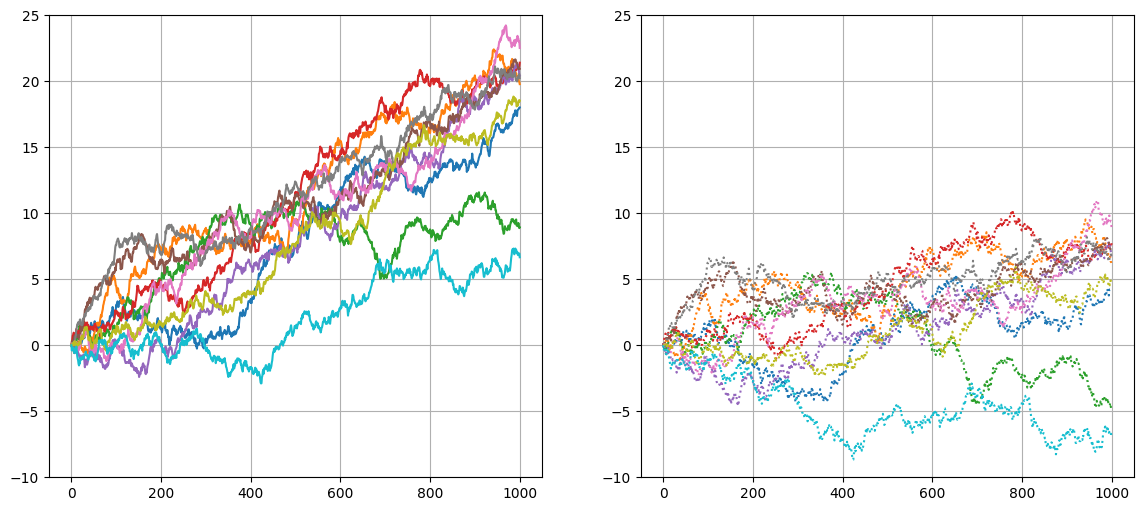
\includegraphics[width=0.5\linewidth]{addons/brownian_motion_girsanov}
%	\end{center}
%	\label{fig:brownian_motion_girsanov}
%\end{figure}
\end{exercise}

\begin{exercise}
Given an underlying asset $S$ which currently is valued 100 simulate $N$ possible realization of the random variable $S$ both under the \emph{physical} probability measure and the 
and a 1 year call option on that asset with strike $K=120$ determine 


mu = 0.05
r = 0.01
sigma = 0.20
l = (mu-r)/sigma
S0 = 100
K = 120
T = 1
M = 252
dt = T/M
N = 10000
%\begin{figure}[htbp]
%	\begin{center}
%		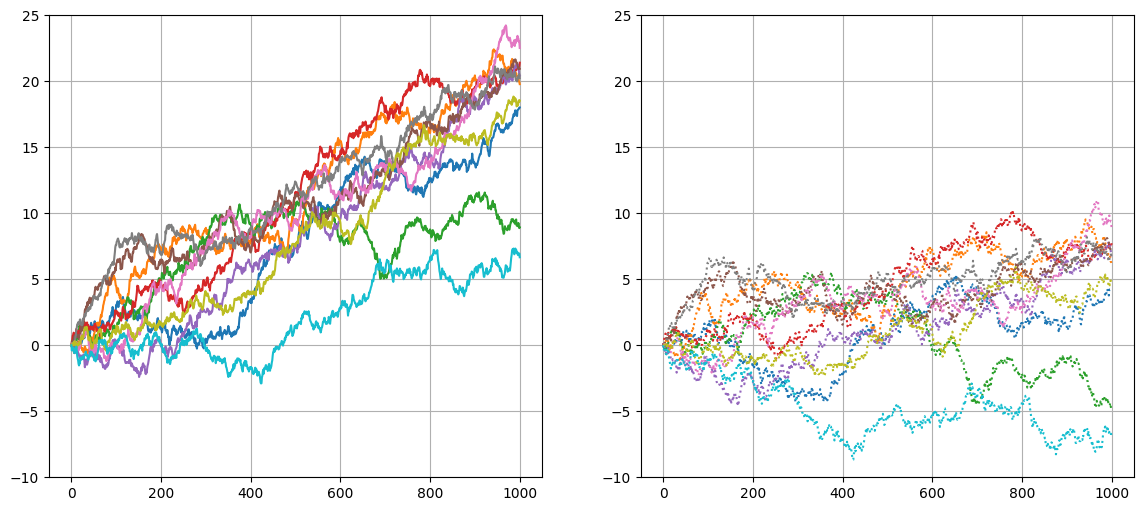
\includegraphics[width=0.5\linewidth]{addons/brownian_motion_girsanov}
%	\end{center}
%	\label{fig:brownian_motion_girsanov}
%\end{figure}
\end{exercise}

\begin{exercise}[subtitle=Moving Away from $\mathbb{P}$ Measure]
Assume that a stock price has the following dynamics (Geometric Brownian Motion) under the real-world measure $\mathbb{P}$
\begin{equation*}
dS_t = \mu S_t dt + \sigma S_t dW_t
\end{equation*}

By definition the bank account dynamics is described by (for simplicity let's consider deterministic rates)
\begin{equation*}
dB_t = rB_tdt\implies B_t = e^{rt}
\end{equation*}

Show what happens to the stock SDE when moving to two different numeraires:
\begin{itemize}
\item risk-neutral measure (bank account numeraire);
\item stock measure (stock numeraire).
\end{itemize}
\end{exercise}

\begin{solution}
%\subsection{Risk-Neutral Measure Dynamics}
We have seen that under the bank account induced measure the process defined as an asset divided by the numeraire is a martingale
\begin{equation*}
\cfrac{S_t}{B_t} = \mathbb{E}^{B}\left[\frac{S_T}{B_T}\bigg|\mathcal{F}_t\right]
\end{equation*}

So if we define $Z_t=\cfrac{S_t}{B_t}$, since $Z_t$ is a martingale (no-drift process) it's evolution could be described by
\begin{equation}
dZ_t = \sigma Z_t dW_t^B
\label{eq:z_martingale1}
\end{equation}
where $dW_t^B$ is a Brownian motion under the $\mathbb{Q}^B$ measure.

Computing directly the $Z_t$ differential (by It$\hat{o}$'s rule at first order)
\begin{equation*}
\begin{aligned}
d\left(\frac{S_t}{B_t}\right) &= \frac{dS_t}{B_t} + S_t d\left(\frac{1}{B_t}\right) = \\ 
&=\frac{dS_t}{B_t} + S_t d\left(e^{-rt}\right) = \frac{dS_t}{B_t} - S_t re^{-rt}dt \\
&= \frac{dS_t}{B_t} - r\frac{S_t}{B_t}dt 
\end{aligned}
\end{equation*}

Now substitute for $dS_t$
\begin{equation*}
d\left(\frac{S_t}{B_t}\right)= \frac{ \mu S_t dt + \sigma S_t dW_t}{B_t} - r\frac{S_t}{B_t}dt = \sigma\frac{S_t}{B_t}\left(\frac{\mu - r}{\sigma}dt + dW_t \right)
\end{equation*}	

In terms of $Z_t$ it becomes
\begin{equation}
dZ_t = \sigma Z_t\left(\frac{\mu - r}{\sigma}dt + dW_t \right)
\label{eq:z_martingale2}
\end{equation}

Both~\ref{eq:z_martingale2} and~\ref{eq:z_martingale1} represent the dynamics of $Z_t$ so they must be equal
\begin{equation*}
\cancel{\sigma Z_t}dW_t^B = \cancel{\sigma Z_t}\left(\frac{\mu - r}{\sigma}dt + dW_t\right)
\end{equation*}
Replacing the Brownian Motion into the real-world dynamics
\begin{equation*}
\begin{aligned}
dS_t &= \mu S_t dt + \sigma S_t \left(dW_t^B - \frac{\mu - r}{\sigma}dt\right) =\\
& = \cancel{\mu S_t dt} \cancel{-\mu S_t dt} + rS_t dt + \sigma S_t dW_t^B  = \boxed{rS_t dt + \sigma S_t dW_t^B}
\end{aligned}
\end{equation*}
So \textbf{under the risk-neutral measure the drift equals the risk-free rate}.

%\subsection{Stock Numeraire Measure Dynamics}
Now let's see what happens under the stock numeraire.
Under the risk-neutral measure $\mathcal{Q}^B$
\begin{equation*}
\frac{S_0}{B_0} = \mathbb{E}^{B}\left[\frac{S_t}{B_t}\bigg|\mathcal{F}_0\right] \implies
S_0 = \mathbb{E}^{B}\left[B_0\frac{S_t}{B_t}\bigg|\mathcal{F}_0\right]
\end{equation*}

By the Change of Numeraire Theorem under the measure $\mathbb{Q}^A$ induced by asset numeraire $A$
\begin{equation*}
S_0 = \mathbb{E}^{A}\left[A_0\frac{S_t}{A_t}\bigg|\mathcal{F}_0\right]
\end{equation*}

Since both expressions represent a price of an asset they must be the same and we can equal the terms inside the expectations. Note that the expectations are computed according two different measures so we keep the factors $d\mathbb{Q}^X$. 

\begin{equation*}
\frac{B_0}{B_t}d\mathbb{Q}^B = \frac{A_0}{A_t}d\mathbb{Q}^A\implies \frac{d\mathbb{Q}^A}{d\mathbb{Q}^B}=\frac{B_0A_t}{B_tA_0}
\end{equation*}
We have already derived the analytical GBM solution in the risk-neutral measure
\begin{equation*} 
A_t = A_0 \exp\left(rt-\frac{1}{2}\sigma^2 t + \sigma W^B_t\right)
\end{equation*}

So we can replace the numeraire definition into the Radon-Nikodym derivative
\begin{equation*}
\frac{d\mathbb{Q}^A}{d\mathbb{Q}^B}=\frac{\cancel{A_0}e^{\cancel{rt}-\frac{1}{2}\sigma^2 t + \sigma W^B_t}}{\cancel{e^{rt}}\cancel{A_0}}=\exp\left(-\frac{1}{2}\sigma^2 t + \sigma W^B_t\right)
\end{equation*}

From the Girsanov theorem, setting the function $\gamma_t = \sigma$, we can get the transformed diffusion process
\begin{equation*}
dW_t^A = dW_t^B - \sigma dt 
\end{equation*}

Substituting back into the risk-neutral dynamics we get
\begin{equation*}
\begin{aligned}
dS_t &= r S_t dt + \sigma S_t dW_t^B = 
rS_t dt + \sigma S_t (dW_t^A + \sigma dt) \\
& = (r + \sigma^2)S_t dt + \sigma S_t dW^A_t
\end{aligned}
\end{equation*}

%\subsection{Summarizing the Results}
To summarize all the results

\begin{table}[htbp]
\begin{center}
\begin{tabular}{llr}
$(i)$&$dS_t = \textcolor{red}{\mu} S_t dt + \sigma S_t dW_t$ & Real-world measure \\
$(ii)$&$dS_t = \textcolor{red}{r}S_t dt + \sigma S_t dW_t^B$ & Risk-neutral measure \\
$(iii)$&$dS_t = \textcolor{red}{(r + \sigma^2)}S_t dt + \sigma S_t dW^A_t$ & Stock measure
\end{tabular}
\end{center}
\end{table}
In practical terms, this means that it possible to use equation $(ii)$, instead of equation $(i)$, to simulate future payoffs, and hence that it is possible to get rid of the big problem of the equity premium estimation. Equation $(ii)$ just needs estimates of the risk-free rate $r$ and of the volatility $\sigma$, which can be derived from real market quotes.
\end{solution}

\chapter{Libor Market Models}
\section{Importance Sampling}
Assume we want to calculate the expectation $\mathbb{E}[f(X)]$
\begin{equation}
\mathbb{E}[f(X)] = \int_{-\infty}^\infty f(x)p(x)dx
\end{equation}
where $p(x)$ is the probability density function associated to the random variable $X$.

We can approximate this expectation using numerical approximation, i.e. Monte Carlo simulation, by sampling $n$ random values from the distribution $p$ and then calculating the sample mean as:
\begin{equation}
\bar{f}(x) = \frac{1}{n}\sum_i f(x_i)
\end{equation}

The idea behind \textbf{importance sampling} is to use a simple re-formulation trick and write the expectation in a slightly different form
\begin{equation}
\mathbb{E}[f(X)] = \int_{-\infty}^\infty f(x)\frac{p(x)}{q(x)}q(x)dx
\end{equation}
giving the expectation of $f(x)\frac{p(x)}{q(x)}$ over the distribution $q$. And with that, allowing us to calculate the sample mean by sampling from $q$:
\begin{equation}
\bar{f}(x) = \frac{1}{n}\sum_i f(x_i)\frac{p(x)}{q(x)}
\label{eq:reformulated_expectation}
\end{equation}

\subsection{Variance Reduction}
From probability theory we know that the variance of the standard Monte Carlo estimator is given by:
\begin{equation}
\cfrac{1}{n}\cdot\text{Var}[f(x)] = \cfrac{1}{n}\cdot\mathbb{E}[(f(X)-\mathbb{E}[f(X)])^2]
\end{equation}

Hence the variance for the re-formulated importance sampling estimator in Eq.~\ref{eq:reformulated_expectation} is:
\begin{equation}
\cfrac{1}{n}\cdot\text{Var}\left[\cfrac{p(x)}{q(x)}f(x)\right]
\end{equation}

This give us a hint o	n how to find a way to reduce the variance. And indeed it is relatively easy to see that this variance could be reduced to 0 by choosing $q$ as:
\begin{equation}
\begin{aligned}
q(x)&=\cfrac{f(X)p(x)}{\mathbb{E}[f(X)]} \implies \cfrac{1}{n}\cdot\text{Var}[\mathbb{E}[f(X)]] = \cfrac{1}{n}\cdot\mathbb{E}[(\mathbb{E}[f(X)]-\mathbb{E}[\mathbb{E}[f(X)]])^2]=\\
&=\cfrac{1}{n}\cdot\mathbb{E}[(\mathbb{E}[f(X)]-\mathbb{E}[f(X)])^2] = 0
\end{aligned}
\end{equation}

Naturally, we don’t know $\mathbb{E}[f(X)]$, as the reason we are doing this sampling after all is to find the expectation of $f$.
However, we can think of the denominator of the previous expression as some normalisation constant, and consider to construct $q$ such that it has \textbf{high} density wherever $f(x)p(x)$ is \textbf{high}.

For the sake of demonstration, we choose $f=\mathcal{N}(5, 1)$, and the probability distribution $p=\mathcal{N}(9,2)$ which do not overlap too well, see Fig.~\ref{fig:f_and_p}.
\begin{figure}[htbp]
\begin{center}
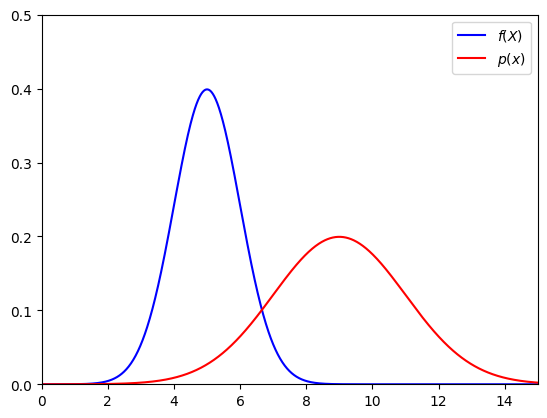
\includegraphics[width=0.5\linewidth]{addons/f_and_p}
\end{center}
\caption{Distributions of the function $f$ and its probability distribution $p$.}
\label{fig:f_and_p}
\end{figure}

To approximate numerically the expectation, as stated above, we would now sample values $x_i$ from the distribution $p$, and compute the mean of $f(x_i)$.

Intuitively one can see why sampling from this distribution is a bad idea: for most values sampled from $p$, $f$ will be close to 0, but for a few sampled values $f$ will be very large, thus we obtain a large variance.

\begin{figure}[htbp]
\begin{center}
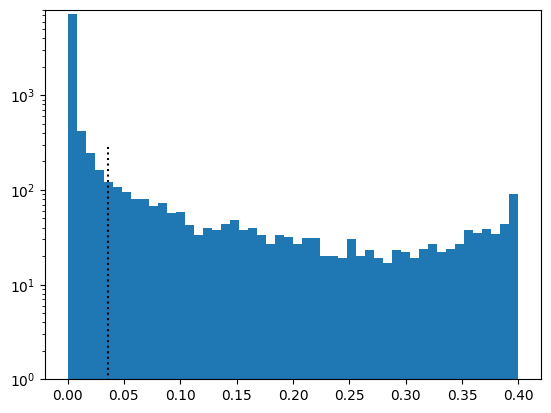
\includegraphics[width=0.5\linewidth]{addons/bad_sampling}
\end{center}
\caption{Distribution of the samples from $f$ with the original probability distribution $p$.}
\label{fig:bad_sampling}
\end{figure}

Looking at Fig.~\ref{fig:bad_sampling} it is apparent how the vast majority of samples piles up at 0 (notice the logarithmic scale of the plot). 
Therefore, as outlined above, to make the sampling more efficient, we can try a new distribution $q = \mathcal{N}(5.8, 1)$, which satisfies the criterion that its pdf is high in regions where $f(x)p(x)$ is high, see Fig.~\ref{fig:fp_and_q}.

\begin{figure}[htbp]
\begin{center}
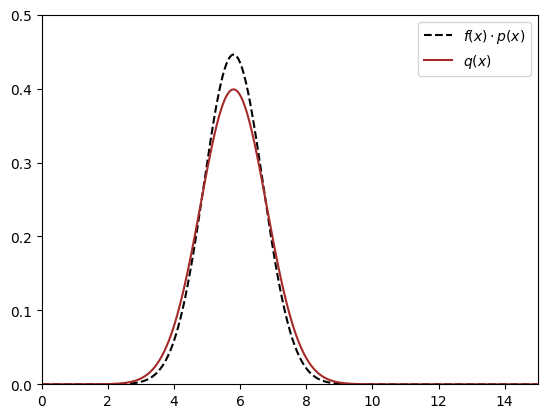
\includegraphics[width=0.4\linewidth]{addons/fp_and_q}
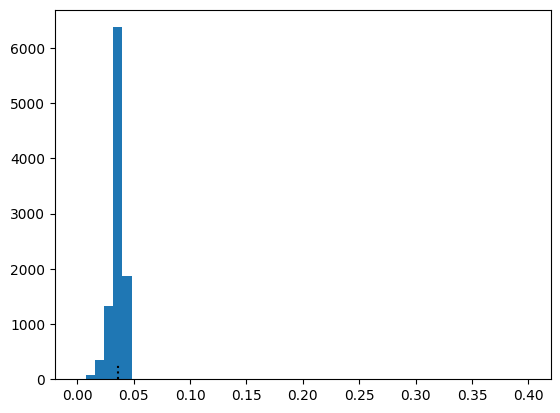
\includegraphics[width=0.4\linewidth]{addons/good_sampling}
\end{center}
\caption{(left) New probability distribution $q$, notice how it almost overlap with $f$. (right) Distribution of the samples from $f$ with the new probability distribution $q$. Now the distribution is way much narrower.}
\label{fig:fp_and_q}
\end{figure}

The resulting sampling is much better since the values are now clustered around 0.03. Comparing the estimates of the expectation in the two cases shows that the value is essentially the same, but the variance almost a factor 200 lower when using the importance sampling.
\begin{ioutput}
Numerical Simulation: mean 0.03611, variance 0.00759
Importance Sampling: mean 0.03603, variance 0.00003
\end{ioutput}
Note that in general it’s not trivial at all to find $q$, and certainly there are much more difficult real-word scenarios. For this example I actually plotted $p(x)f(x)$ and then picked a $q$ which resembled it best.

\begin{exercise}
Implement the importance sampling example outlined above, trying to reproduce the results quoted in the text.
\end{exercise}

\begin{exercise}[subtitle=How Unlucky is Unlucky]
Estimate how unlucky is a 25 standard deviation return
\begin{equation*}
\theta := P(X\geq 25) = \mathbb{E}[\mathbbm{1}_{X\geq 25}]  \quad\text{where } X\sim \mathcal{N}(0, 1)
\end{equation*}
\end{exercise}

\begin{exercise}[subtitle=Importance Sampling and Black-Scholes]
Consider a one year ($T=1$) call option with $S_0=100$ , $K=170$,  $\sigma=0.2$, and $r=0.06$. The option is far out of the money, assuming we need to estimate its value using Monte Carlo simulation, improve the efficiency of the calculation with importance sampling.

\noindent
Interesting reference \emph{Variance Reduction Techniques of Importance Sampling Monte Carlo Methods for Pricing Options}, 
Journal of Mathematical Finance, 2013, 3, 431-436.
\end{exercise}

%\section{Principal Component Analysis}
%Principal component analysis (PCA) is a dimension reduction technique in multivariate analysis. It can be used for constructing the components of the stochastic term-structure movements that account for most of the variability, in some appropriately defined sense.
%
%The key mathematical principle behind PCA is the spectral decomposition theorem of linear algebra, which states that any real symmetric $n\times n$ matrix $Q$ can be written as
%\begin{equation}
%Q = ALA^{T}
%\label{eq:spectral_decomposition}
%\end{equation}
%where: $L = \text{diag}(\lambda_1,\ldots, \lambda_n$) is the diagonal matrix of eigenvalues of $Q$ with $\lambda_1 \geq \lambda_2 \geq \cdots \geq \lambda_n$, $A$ is an orthogonal matrix (that is, $A^{-1}=A^{T}$) whose columns $a_1,\ldots, a_n$ are the normalized eigenvectors of $Q$ (that is, $Qa_i = \lambda_i a_i$), which form a \emph{basis}.
%
%Consider a random vector $X$ with mean $\mu = \mathbb{E}[X]$ and covariance matrix $Q = \text{Cov}[X]$. Since $Q$ is symmetric and positive semi-definite,
%the above decomposition Eq.~v\ref{eq:spectral_decomposition} applies with $\lambda_i\geq 0$ for all $i$. The principal components transform of X is defined as
%\begin{equation}
%Y = A^{T}(X -\mu)
%\end{equation}
%which can be seen as a recentering and rotation of $X$. Note that each $Y_i$ is the projection of $(X-\mu)$ onto the $i$th eigenvector $a_i$ of $Q$ which can be called the $i$th principal component, and $a_i$, the $i$th vector of loadings, fo $X$. We thus obtain the decomposition
%\begin{equation}
%X = \mu + AY = \mu + \sum_{i=1}^n Y_i a_i
%\end{equation}
%
%It can be demonstrated that 
%\begin{equation}
%\sum_{i=1}^n\text{Var}[X_i] = \sum_{i=1}^n\text{Var}[\lambda_i] = \sum_{i=1}^n\text{Var}[Y_i]
%\end{equation}
%hence
%\begin{equation}
%\cfrac{\sum_{i=1}^k\text{Var}[\lambda_i]}{\sum_{i=1}^n\text{Var}[\lambda_i]}
%\end{equation}
%represents the amount of variability in $X$ explained byt the first $k$ principal components $Y_1,\ldots,Y_k$.
%
%Suppose that the first $k$ principal components $Y_1,\ldots,Y_k$ explain a significant amount (e.g. 99\%) of the variability in $X$. It is then most useful to
%approximate $X$ by $X\approx\mu +\sum_{i=1}^{k}Y_ia_i$. That is, the loadings $a_1,\ldots, a_k$ are the main components of the stochastic forward curve movements.
%v
%\begin{exercise}
%The Excel file \href{https://github.com/matteosan1/finance_course/raw/develop/input_files/SNB_yields.xlsx}{SNB\_yields.xls} of the Monthly Statistical Bulletin from the Swiss National Bank contains monthly spot interest rates (that is, yields $R(t,T)$) for Swiss Confederation bonds for a time to maturity $(T-t)$ spectrum of 2, 3, 4, 5, 7, 10, 20 and 30 years. 
%Perform a principal component analysis of the monthly yield curve changes for the forward curve from the last ten years. In particular, determine:
%\begin{enumerate}
%\item the empirical covariance matrix;
%\item its eigenvectors and eigenvalues in decreasing order;
%\item the explained variances of the principal components.
%\end{enumerate}
%\end{exercise}

\tableofcontents

\chapter*{Solutions}
\printsolutions*[chapter=1, headings-template=per-chapter]
\printsolutions*[chapter=2, headings-template=per-chapter]
\printsolutions*[chapter=3, headings-template=per-chapter]
\printsolutions*[chapter=4, headings-template=per-chapter]
\printsolutions*[chapter=5, headings-template=per-chapter]

\end{document}
